\documentclass[12pt, a4paper]{article}

% ==========================================
% 1. KHAI BÁO GÓI THƯ VIỆN (PACKAGES)
% ==========================================
% Bảng mã & Font chữ
\usepackage[utf8]{inputenc}
\usepackage[T5]{fontenc}

% Toán học
\usepackage{amsmath, amssymb}


% Căn lề & Bố cục trang
\usepackage[top=2.2cm, bottom=1.5cm, left=1cm, right=1cm, headheight=15pt]{geometry}
\usepackage{fancyhdr}
\usepackage{needspace}
\usepackage{tkz-tab}

% Đồ họa & Màu sắc
\usepackage{xcolor}
\usepackage{graphicx} 
\usepackage{tikz}
\usetikzlibrary{calc, shapes.geometric, positioning}


% Bảng biểu & Danh sách
\usepackage{colortbl}
\usepackage{array}
\usepackage{makecell}
\usepackage{multirow}
\usepackage{tasks}

% Biểu tượng
\usepackage{fontawesome5}

% ==========================================
% 2. THIẾT LẬP MÀU SẮC CHỦ ĐẠO
% ==========================================
\definecolor{goldyellow}{RGB}{255, 179, 0}
\definecolor{amberorange}{RGB}{230, 115, 0}
\definecolor{lightamber}{RGB}{255, 248, 225}
\definecolor{deepblue}{RGB}{25, 42, 86}
\definecolor{accentred}{RGB}{232, 65, 24}
\definecolor{softgray}{RGB}{220, 220, 222} 
\definecolor{fbblue}{RGB}{15, 80, 200}


% ==========================================
% 3. CẤU HÌNH HEADER & FOOTER
% ==========================================
\pagestyle{fancy}
\fancyhf{}
\renewcommand{\headrulewidth}{0pt}

% Khai báo biến lưu trữ nội dung góc phải của Header
\newcommand{\HeaderRightText}{}

% --- Header ---
\fancyhead[C]{
    \begin{tikzpicture}[remember picture, overlay]
        
        % Dải màu trang trí góc trên
        \path[fill=deepblue] (current page.north west) -- (current page.north east) 
            -- ($(current page.north east) + (0, -1.6cm)$) 
            .. controls ($(current page.north) + (3, -2.0cm)$) and ($(current page.north) + (-3, -0.4cm)$) .. 
            ($(current page.north west) + (0, -1.0cm)$) -- cycle;
            
        \path[fill=goldyellow] (current page.north west) -- (current page.north east) 
            -- ($(current page.north east) + (0, -1.0cm)$) 
            .. controls ($(current page.north) + (4, -1.0cm)$) and ($(current page.north) + (-2, -2.2cm)$) .. 
            ($(current page.north west) + (0, -1.6cm)$) -- cycle;
            
        \path[fill=amberorange] (current page.north west) -- ($(current page.north west) + (6.5cm, 0)$) 
            .. controls ($(current page.north west) + (4.5cm, -1.2cm)$) and ($(current page.north west) + (2cm, -2.0cm)$) .. 
            ($(current page.north west) + (0, -2.0cm)$) -- cycle;
            
        % Logo góc trái Header
        \node[anchor=west, inner sep=0pt] 
            at ($(current page.north west) + (0cm, -0.8cm)$) {
\includegraphics[height=2.0cm]{../../../image/logo-header.png}};
            
        % Text góc phải Header (Tự động lấy từ đối số thứ 3 của \titlebox)
        \node[anchor=east, text=white, font=\small\bfseries\sffamily] 
            at ($(current page.north east) + (-0.8cm, -0.5cm)$) {\HeaderRightText};
    \end{tikzpicture}
}

% --- Footer ---
\fancyfoot[C]{
    \begin{tikzpicture}[remember picture, overlay]
        % Đường kẻ ngang
        \draw[amberorange, line width=1.5pt] 
            ($(current page.south west) + (0cm, 0.4cm)$) -- ($(current page.south east) + (0cm, 0.4cm)$);

        % Dải cong góc phải
        \path[fill=goldyellow] (current page.south east) -- ($(current page.south east) + (-5cm, 0)$) 
            .. controls ($(current page.south east) + (-3cm, 0.8cm)$) and ($(current page.south east) + (-1.5cm, 1.2cm)$) .. 
            ($(current page.south east) + (0, 1.2cm)$) -- cycle;

        % Mạng xã hội
        \node[anchor=west, inner sep=0pt] at ($(current page.south west) + (1cm, 0.8cm)$) {
            \small\sffamily
            \textcolor{fbblue}{\faFacebook\hskip 4pt Toán Anh Huy MATH-STER}
            \hskip 18pt
            \textcolor{black}{\faTiktok\hskip 4pt huymathster}
        };

        % Số trang (Thiết kế hình tròn cũ thu nhỏ)
        \node[circle, fill=white, draw=amberorange, line width=1.5pt, text=deepblue, font=\large\bfseries, inner sep=0pt, minimum size=0.7cm] 
            at ($(current page.south east) + (-1.0cm, 0.65cm)$) {\thepage};
    \end{tikzpicture}
}

% ==========================================
% 4. ĐỊNH NGHĨA MACRO: KHUNG TIÊU ĐỀ
% ==========================================
\newcommand{\titlebox}[3]{
    % Gán nội dung đối số #3 vào biến HeaderRightText
    \gdef\HeaderRightText{#3}
    
    \begin{center}
    \vspace*{-0.5cm}
    \begin{tikzpicture}
        % Khung vô hình (Phantom Box) định chuẩn kích thước
        \node[text width=16cm, inner xsep=0pt, inner ysep=16pt, opacity=0] (MainBox) {
            \begin{minipage}[c]{4.2cm}
                \centering\vspace{0.1cm}
                \rule{2.2cm}{2.2cm} 
                \vspace{0.1cm}
            \end{minipage}%
            \begin{minipage}[c]{11.5cm}
                \centering\vspace{0.15cm}
                {\huge\bfseries\sffamily #2 \par}
                \vspace{0.15cm} 
            \end{minipage}
        };
        
        % Đổ bóng & Nền
        \fill[goldyellow, rounded corners=8pt] ([xshift=5pt, yshift=-5pt]MainBox.south west) rectangle ([xshift=5pt, yshift=-5pt]MainBox.north east);
        \fill[white, rounded corners=8pt] (MainBox.south west) rectangle (MainBox.north east);
        
        % Lưới ô ly & Nền Logo
        \begin{scope}
            \clip[rounded corners=8pt] (MainBox.south west) rectangle (MainBox.north east);
            \draw[step=0.4cm, softgray!50, line width=0.6pt] (MainBox.south west) grid (MainBox.north east);
            \fill[lightamber!60] (MainBox.south west) rectangle ([xshift=4.2cm]MainBox.north west);
        \end{scope}

        % Viền ngoài
        \draw[deepblue, line width=1.5pt, rounded corners=8pt] (MainBox.south west) rectangle (MainBox.north east);

        % Nội dung Text (Lớp trên cùng)
        \node[text width=16cm, inner xsep=0pt, inner ysep=16pt] at (MainBox.center) {
            \begin{minipage}[c]{4.2cm}
                \centering
                % --- ĐIỀU CHỈNH TỌA ĐỘ LOGO Ở ĐÂY ---
                \hspace*{-0.5cm}\raisebox{-0.2cm}{
\includegraphics[width=5.5cm]{../../../image/logo.png}}
            \end{minipage}%
            \begin{minipage}[c]{11.5cm}
                \centering\vspace{0.15cm}
                {\huge\bfseries\sffamily\color{deepblue} #2 \par}
                \vspace{0.15cm} 
            \end{minipage}
        };
        
        % Trang trí phụ kiện
        \draw[deepblue, line width=1.5pt, dashed] ([xshift=4.2cm]MainBox.north west) -- ([xshift=4.2cm]MainBox.south west);
        \node[regular polygon, regular polygon sides=4, rotate=45, fill=white, draw=accentred, line width=1.2pt, inner sep=2.5pt] at ([xshift=4.2cm]MainBox.west) {};
        \node[anchor=west, fill=amberorange, text=white, font=\large\bfseries\sffamily, rounded corners=4pt, draw=deepblue, line width=1.5pt, inner xsep=12pt, inner ysep=6pt] at ([xshift=1.5cm]MainBox.north west) {#1};
        \fill[accentred] ([xshift=-1.8cm, yshift=-0.4cm]MainBox.north east) circle (3pt);
        \fill[amberorange] ([xshift=-1.4cm, yshift=-0.4cm]MainBox.north east) circle (3pt);
        \fill[goldyellow] ([xshift=-1.0cm, yshift=-0.4cm]MainBox.north east) circle (3pt);
    \end{tikzpicture}
    \vspace*{0cm}
    \end{center}
}

% ==========================================
% 5. ĐỊNH NGHĨA MACRO: CẤU TRÚC CÂU HỎI (ÉP SÁT NHAU)
% ==========================================
\newcommand{\questioncore}[2]{
    % Xóa khoảng cách phía trên, ép sát câu trước
    \noindent \textbf{\textcolor{deepblue}{Câu #1.} \textcolor{accentred}{[STER]}} #2
    \par\nopagebreak
}

% Cấu hình hiển thị đáp án trắc nghiệm
\settasks{
    label=\textbf{\textcolor{amberorange}{\Alph*.}}, 
    label-width=15pt,     
    item-indent=25pt,     
    label-offset=6pt,    
    column-sep=20pt,     
    after-item-skip=2pt  % Đã giảm tối đa khoảng cách giữa các dòng đáp án A B C D
}

% Hàm vẽ dòng kẻ nháp
\newcommand{\drawdashlines}[1]{
    \ifnum#1>0
        \nopagebreak\vspace{0.1cm}\noindent 
        \begin{tikzpicture}
            \foreach \i in {1,...,#1} {
                \draw[softgray, line width=0.2pt] (0,-{\i*0.75}) -- (\textwidth-4pt,-{\i*0.75});
            }
        \end{tikzpicture}
        \par
    \fi
    % Đã xóa hoàn toàn khoảng cách thừa ở nhánh else
}

% --- Dạng 1: Trắc nghiệm 4 đáp án ---
\newcommand{\questionLinesManual}[4]{
    \pgfmathsetmacro{\calculatedSpace}{1.5 + #1 * 0.65}
    \needspace{\calculatedSpace cm} 
    \questioncore{#2}{#3}
    #4
    \par\nopagebreak
    \drawdashlines{#1}
}

% --- Dạng 2: Trắc nghiệm Đúng/Sai ---
\newcommand{\questionTrueFalse}[4]{
    \pgfmathsetmacro{\calculatedSpace}{3.0 + #1 * 0.65} 
    \needspace{\calculatedSpace cm}
    \questioncore{#2}{#3}
    
    \nopagebreak
    \begin{center}
    \renewcommand{\arraystretch}{1.2} % Bóp nhỏ chiều cao của bảng Đ/S
    \begin{tabular}{|>{\centering\arraybackslash}m{0.8cm}|m{12cm}|>{\centering\arraybackslash}m{2cm}|>{\centering\arraybackslash}m{2cm}|}
        \hline
        \rowcolor{amberorange!20}
        & \multicolumn{1}{>{\centering\arraybackslash}m{12cm}|}{\textbf{\textcolor{deepblue}{Mệnh đề}}} & 
        \textbf{\textcolor{deepblue}{Đúng}} & 
        \textbf{\textcolor{deepblue}{Sai}} \\
        \hline
        #4
        \hline
    \end{tabular}
    \renewcommand{\arraystretch}{1}
    \end{center}
    
    \par\nopagebreak
    \drawdashlines{#1}
}

% ----- Dạng 3: Tự luận ngắn -----
\newcommand{\questionShortAnswer}[3]{
    \pgfmathsetmacro{\calculatedSpace}{1.5 + #1 * 0.8}
    \needspace{\calculatedSpace cm}
    
    {\linespread{1.1}\selectfont % Bóp nhỏ giãn dòng của câu tự luận
    \questioncore{#2}{#3}\par}
    
    \nopagebreak
    \begin{flushright}
        \begin{tikzpicture}
            \node[anchor=east, font=\small\bfseries\sffamily, text=deepblue] 
                at (-0.2, 0.4) {Đáp án:};
            \fill[goldyellow, rounded corners=3pt] (0.08, -0.08) rectangle (3.08, 0.72);
            \draw[draw=deepblue, fill=white, line width=1.2pt, rounded corners=3pt] 
                (0,0) rectangle (3.0, 0.8);
            \foreach \x in {0.75, 1.5, 2.25} {
                \draw[draw=deepblue, line width=0.6pt] (\x, 0) -- (\x, 0.8);
            }
        \end{tikzpicture}
    \end{flushright}
    
    \par\nopagebreak
    \drawdashlines{#1}
}

% ==========================================
% BẮT ĐẦU NỘI DUNG TÀI LIỆU
% ==========================================
\begin{document}

% Truyền 3 tham số: {Nhãn cam} {Chữ to chính giữa} {Chữ ở góc phải Header}
\titlebox{Chủ đề: Hàm số}{Cực trị của hàm số}{Hàm số: Cực trị}
% ====== CÂU 1 ======
\questionLinesManual{5}{1}{Cho hàm số bậc ba \( y = f(x) \) có bảng biến thiên như sau:
\begin{center}
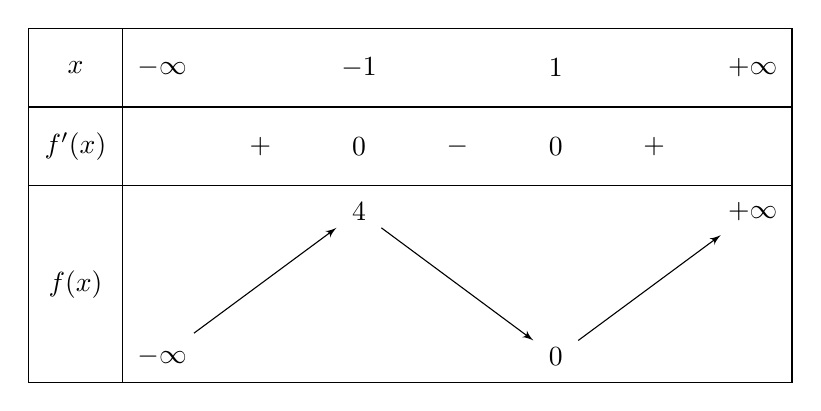
\begin{tikzpicture}[>=stealth]
    \tkzTabInit[nocadre=false,lgt=1.2,espcl=2.5]
    {$x$ / 1, $f'(x)$ / 1, $f(x)$ / 2.5}
    {$-\infty$, $-1$, $1$, $+\infty$}
    \tkzTabLine{ , +, 0, -, 0, + }
    \tkzTabVar{-/$-\infty$, +/$4$, -/$0$, +/$+\infty$}

\end{tikzpicture}
\end{center}
Điểm cực tiểu của đồ thị hàm số là:}{%
\begin{tasks}(4)
\task \((-1; 0)\)
\task \((1; 0)\)
\task \((-1; 4)\)
\task \((1; 4)\)
\end{tasks}
}


% ====== CÂU 2 ======
\questionLinesManual{5}{2}{Cho hàm số \( f(x) \) có bảng biến thiên như sau:
\begin{center}
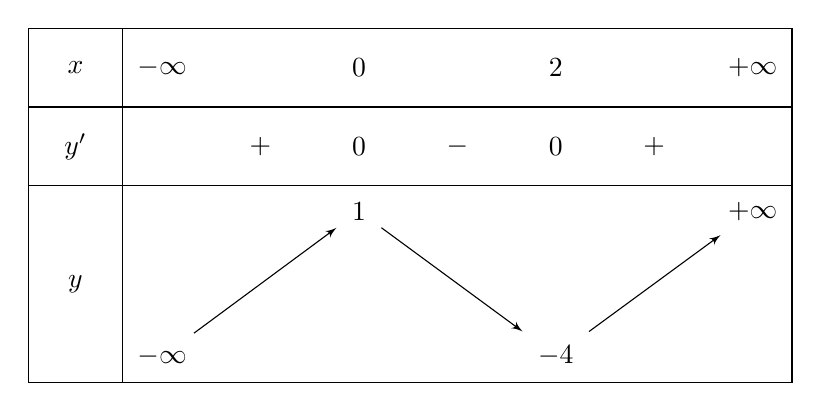
\begin{tikzpicture}[>=stealth]
    \tkzTabInit[nocadre=false,lgt=1.2,espcl=2.5]
    {$x$ / 1, $y'$ / 1, $y$ / 2.5}
    {$-\infty$, $0$, $2$, $+\infty$}
    \tkzTabLine{ , +, 0, -, 0, + }
    \tkzTabVar{-/$-\infty$, +/$1$, -/$-4$, +/$+\infty$}

\end{tikzpicture}
\end{center}
Hàm số đã cho đạt cực tiểu tại điểm nào sau đây?}{%
\begin{tasks}(4)
\task \( x = -4 \)
\task \( x = 2 \)
\task \( x = 1 \)
\task \( x = 0 \)
\end{tasks}
}

% ====== CÂU 3 ======
\questionLinesManual{5}{3}{Cho hàm số \( y = f(x) \) có bảng biến thiên sau:
\begin{center}
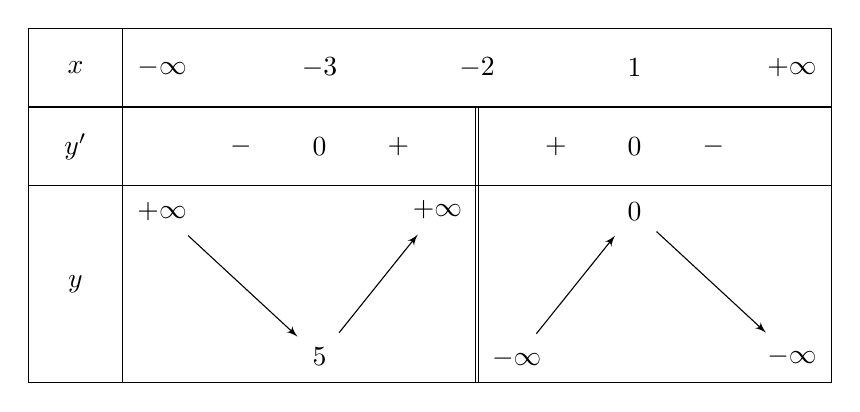
\begin{tikzpicture}[>=stealth]
    \tkzTabInit[nocadre=false,lgt=1.2,espcl=2]
    {$x$ / 1, $y'$ / 1, $y$ / 2.5}
    {$-\infty$, $-3$, $-2$, $1$, $+\infty$}
    \tkzTabLine{ , -, 0, +, d, +, 0, - }
    \tkzTabVar{+/$+\infty$, -/$5$,+D-/$+\infty$ /$-\infty$, +/$0$, -/$-\infty$}

\end{tikzpicture}
\end{center}
Giá trị cực đại của hàm số \( y = f(x) \) là:}{%
\begin{tasks}(4)
\task 0
\task 1
\task $-3$
\task 5
\end{tasks}
}

% ====== CÂU 4 ======
\questionLinesManual{5}{4}{Cho hàm số \( y = f(x) = \dfrac{mx^2 + nx + p}{qx + r} \) có bảng biến thiên như hình vẽ bên dưới.
\begin{center}
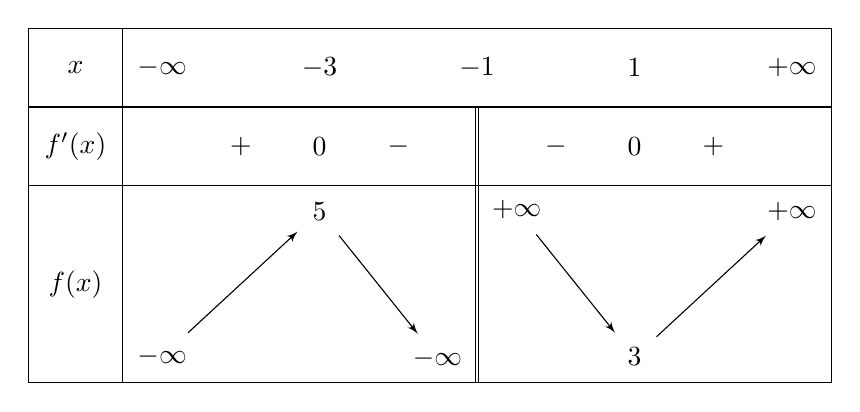
\begin{tikzpicture}[>=stealth]
    \tkzTabInit[nocadre=false,lgt=1.2,espcl=2]
    {$x$ / 1, $f'(x)$ / 1, $f(x)$ / 2.5}
    {$-\infty$, $-3$, $-1$, $1$, $+\infty$}
    \tkzTabLine{ , +, 0, -, d, -, 0, + }
    \tkzTabVar{-/$-\infty$, +/$5$,-D+/$-\infty$ /$+\infty$, -/$3$, +/$+\infty$}

\end{tikzpicture}
\end{center}
Giá trị cực đại của hàm số đã cho bằng}{%
\begin{tasks}(4)
\task 3
\task $-3$
\task $-5$
\task 1
\end{tasks}
}
% ====== CÂU 5 ======
\questionLinesManual{5}{5}{Cho hàm số \( y = f(x) \) có bảng biến thiên như sau:
\begin{center}
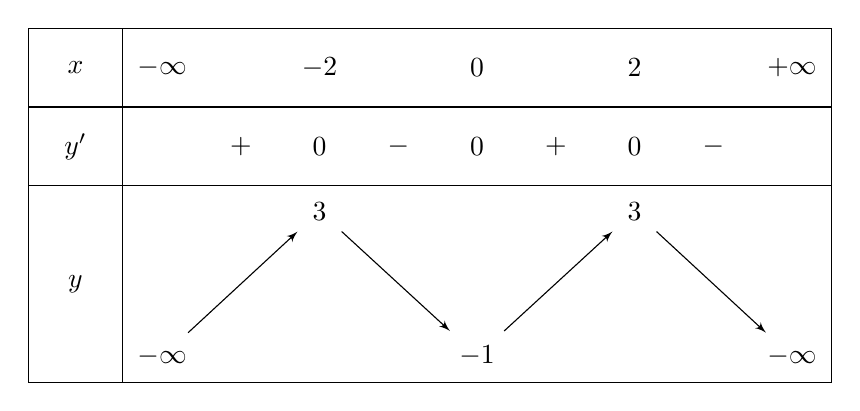
\begin{tikzpicture}[>=stealth]
    \tkzTabInit[nocadre=false,lgt=1.2,espcl=2]
    {$x$ / 1, $y'$ / 1, $y$ / 2.5}
    {$-\infty$, $-2$, $0$, $2$, $+\infty$}
    \tkzTabLine{ , +, 0, -, 0, +, 0, - }
    \tkzTabVar{-/$-\infty$, +/$3$, -/$-1$,+/$3$, -/$-\infty$}

\end{tikzpicture}
\end{center}
Mệnh đề nào sau đây \textbf{sai}?}{%
\begin{tasks}(2)
\task Hàm số có giá trị cực tiểu bằng $-1$.
\task Hàm số có 3 điểm cực trị.
\task Hàm số có giá trị cực đại bằng $-1$.
\task Hàm số có 2 điểm cực đại.
\end{tasks}
}

% ====== CÂU 6 ======
\questionLinesManual{5}{6}{Cho hàm số \( y = f(x) \) có bảng biến thiên như sau:
\begin{center}
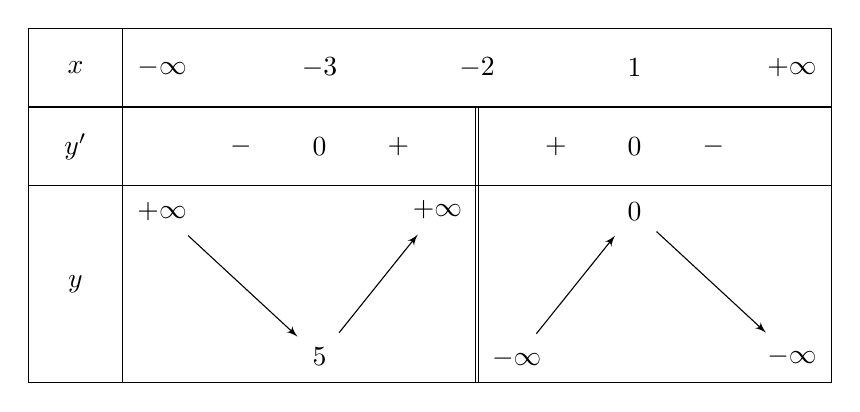
\begin{tikzpicture}[>=stealth]
    \tkzTabInit[nocadre=false,lgt=1.2,espcl=2]
    {$x$ / 1, $y'$ / 1, $y$ / 2.5}
    {$-\infty$, $-3$, $-2$, $1$, $+\infty$}
    \tkzTabLine{ , -, 0, +, d, +, 0, - }
    \tkzTabVar{+/$+\infty$, -/$5$,+D-/$+\infty$ /$-\infty$, +/$0$, -/$-\infty$}
\end{tikzpicture}
\end{center}
Giá trị cực đại của hàm số \( y = f(x) \) là:}{%
\begin{tasks}(4)
\task 0
\task 1
\task $-3$
\task 5
\end{tasks}
}

% ====== CÂU 7 ======
\questionLinesManual{5}{7}{Cho hàm số \( y = f(x) \) có bảng biến thiên sau:
\begin{center}
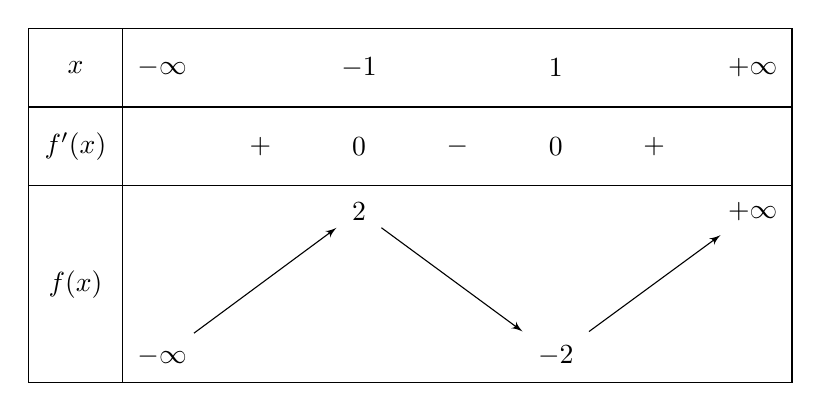
\begin{tikzpicture}[>=stealth]
    \tkzTabInit[nocadre=false,lgt=1.2,espcl=2.5]
    {$x$ / 1, $f'(x)$ / 1, $f(x)$ / 2.5}
    {$-\infty$, $-1$, $1$, $+\infty$}
    \tkzTabLine{ , +, 0, -, 0, + }
    \tkzTabVar{-/$-\infty$, +/$2$, -/$-2$,+/$+\infty$}
\end{tikzpicture}
\end{center}
Giá trị cực tiểu của hàm số đã cho bằng:}{%
\begin{tasks}(4)
\task 2
\task $-2$
\task $-1$
\task 1
\end{tasks}
}
% ====== CÂU 8 ======
\questionLinesManual{5}{8}{Cho hàm số có bảng biến thiên như sau:
\begin{center}
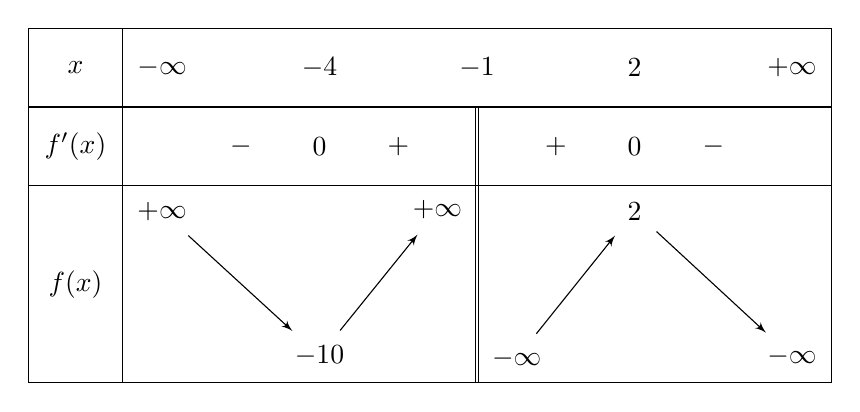
\begin{tikzpicture}[>=stealth]
    \tkzTabInit[nocadre=false,lgt=1.2,espcl=2]
    {$x$ / 1, $f'(x)$ / 1, $f(x)$ / 2.5}
    {$-\infty$, $-4$, $-1$, $2$, $+\infty$}
    \tkzTabLine{ , -, 0, +, d, +, 0, - }
    \tkzTabVar{+/$+\infty$, -/$-10$,+D-/$+\infty$ /$-\infty$, +/$2$, -/$-\infty$}
\end{tikzpicture}
\end{center}
Giá trị cực tiểu của hàm số là}{%
\begin{tasks}(4)
\task 2
\task $-2$
\task $-4$
\task $-10$
\end{tasks}
}

% ====== CÂU 9 ======
\questionLinesManual{5}{9}{Cho hàm số \( f(x) = \dfrac{ax^2 + bx + c}{ex + f} \) có bảng biến thiên như hình sau:
\begin{center}
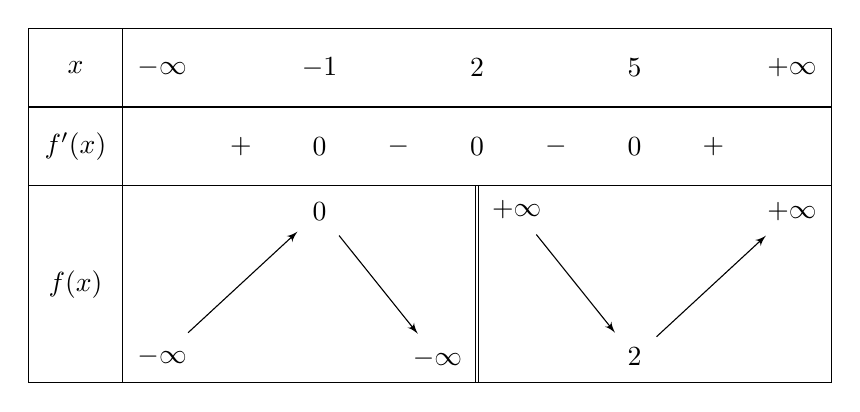
\begin{tikzpicture}[>=stealth]
    \tkzTabInit[nocadre=false,lgt=1.2,espcl=2]
    {$x$ / 1, $f'(x)$ / 1, $f(x)$ / 2.5}
    {$-\infty$, $-1$, $2$, $5$, $+\infty$}
    \tkzTabLine{ , +, 0, -, 0, -, 0, + }
    \tkzTabVar{-/$-\infty$, +/$0$,-D+/$-\infty$ /$+\infty$, -/$2$, +/$+\infty$}
\end{tikzpicture}
\end{center}
Hàm số đã cho đạt cực đại tại điểm}{%
\begin{tasks}(4)
\task \( x = 5 \)
\task \( x = 2 \)
\task \( x = 0 \)
\task \( x = -1 \)
\end{tasks}
}

% ====== CÂU 10 ======
\questionLinesManual{5}{10}{Cho hàm số \( y = f(x) \) xác định trên \( \mathbb{R} \) và có bảng biến thiên như sau:
\begin{center}
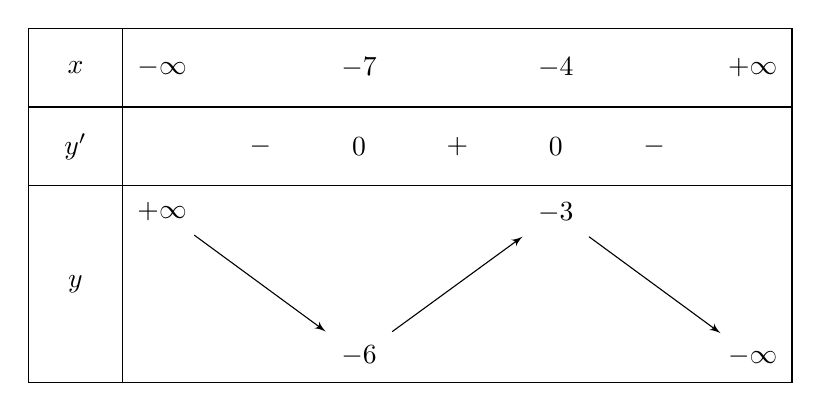
\begin{tikzpicture}[>=stealth]
    \tkzTabInit[nocadre=false,lgt=1.2,espcl=2.5]
    {$x$ / 1, $y'$ / 1, $y$ / 2.5}
    {$-\infty$, $-7$, $-4$, $+\infty$}
    \tkzTabLine{ , -, 0, +, 0, - }
    \tkzTabVar{+/$+\infty$, -/$-6$, +/$-3$,-/$-\infty$}
\end{tikzpicture}
\end{center}
Điểm cực đại của hàm số \( y = f(x) \) là}{%
\begin{tasks}(4)
\task \( x = -7 \)
\task \( x = -6 \)
\task \( x = -3 \)
\task \( x = -4 \)
\end{tasks}
}

% ====== CÂU 11 ======
\questionLinesManual{5}{11}{Cho hàm số bậc ba \( y = f(x) \) có bảng biến thiên như hình vẽ bên dưới
\begin{center}
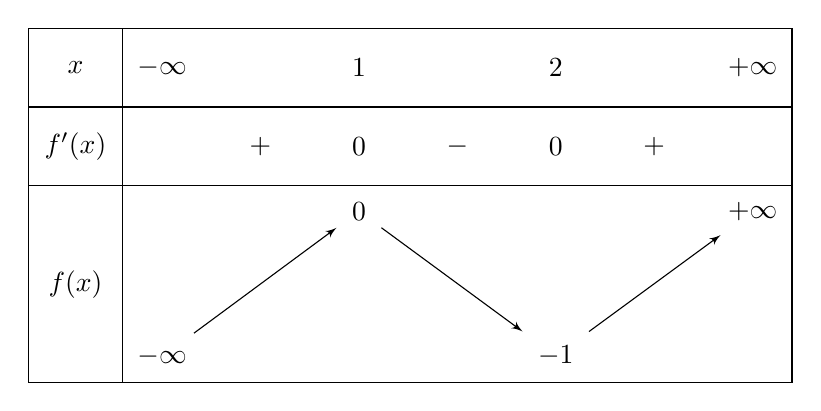
\begin{tikzpicture}[>=stealth]
    \tkzTabInit[nocadre=false,lgt=1.2,espcl=2.5]
    {$x$ / 1, $f'(x)$ / 1, $f(x)$ / 2.5}
    {$-\infty$, $1$, $2$, $+\infty$}
    \tkzTabLine{ , +, 0, -, 0, + }
    \tkzTabVar{-/$-\infty$, +/$0$, -/$-1$,+/$+\infty$}
\end{tikzpicture}
\end{center}
Hàm số đã cho đạt giá trị cực đại tại điểm:}{%
\begin{tasks}(4)
\task \( x = -1 \)
\task \( x = 0 \)
\task \( x = 2 \)
\task \( x = 1 \)
\end{tasks}
}

% ====== CÂU 12 ======
\questionLinesManual{5}{12}{Cho hàm số \( y = f(x) \) xác định và liên tục trên \( \mathbb{R} \) và có bảng biến thiên như sau:
\begin{center}
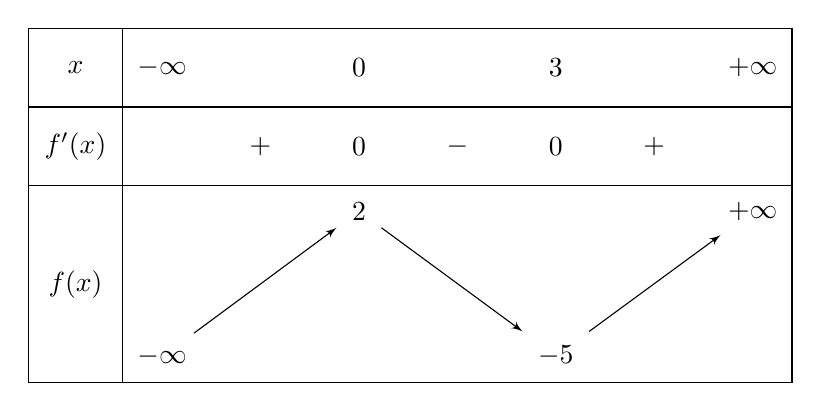
\begin{tikzpicture}[>=stealth]
    \tkzTabInit[nocadre=false,lgt=1.2,espcl=2.5]
    {$x$ / 1, $f'(x)$ / 1, $f(x)$ / 2.5}
    {$-\infty$, $0$, $3$, $+\infty$}
    \tkzTabLine{ , +, 0, -, 0, + }
    \tkzTabVar{-/$-\infty$, +/$2$, -/$-5$,+/$+\infty$}
\end{tikzpicture}
\end{center}
Tổng giá trị cực đại và giá trị cực tiểu của hàm số đã cho bằng bao nhiêu?}{%
\begin{tasks}(4)
\task $-3$
\task $2$
\task $3$
\task $-5$
\end{tasks}
}

% ====== CÂU 13 ======
\questionLinesManual{5}{13}{Cho hàm số \( y = f(x) \) xác định, liên tục trên \( \mathbb{R} \) và có bảng biến thiên như sau:
\begin{center}
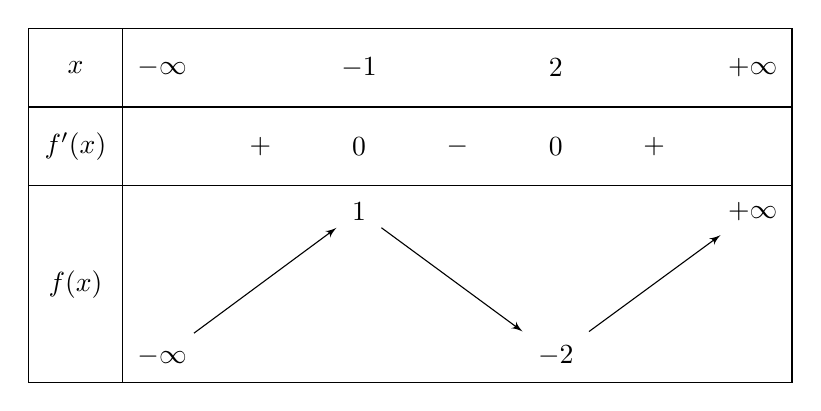
\begin{tikzpicture}[>=stealth]
    \tkzTabInit[nocadre=false,lgt=1.2,espcl=2.5]
    {$x$ / 1, $f'(x)$ / 1, $f(x)$ / 2.5}
    {$-\infty$, $-1$, $2$, $+\infty$}
    \tkzTabLine{ , +, 0, -, 0, + }
    \tkzTabVar{-/$-\infty$, +/$1$, -/$-2$,+/$+\infty$}
\end{tikzpicture}
\end{center}
Điểm nào dưới đây là điểm cực tiểu của hàm số đã cho?}{%
\begin{tasks}(4)
\task \( x = -2 \)
\task \( y = -2 \)
\task \( x = 2 \)
\task \( 2; -2 \)
\end{tasks}
}

% ====== CÂU 14 ======
\questionLinesManual{5}{14}{Cho hàm số \( y = f(x) \) có bảng biến thiên như sau:
\begin{center}
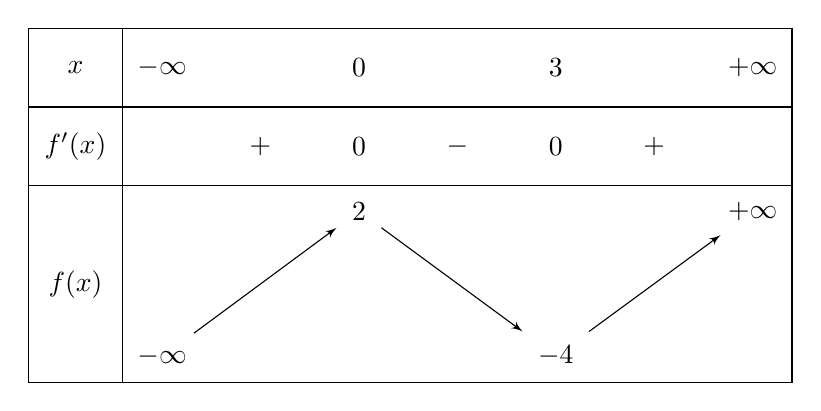
\begin{tikzpicture}[>=stealth]
    \tkzTabInit[nocadre=false,lgt=1.2,espcl=2.5]
    {$x$ / 1, $f'(x)$ / 1, $f(x)$ / 2.5}
    {$-\infty$, $0$, $3$, $+\infty$}
    \tkzTabLine{ , +, 0, -, 0, + }
    \tkzTabVar{-/$-\infty$, +/$2$, -/$-4$,+/$+\infty$}
\end{tikzpicture}
\end{center}
Giá trị cực tiểu của hàm số đã cho bằng}{%
\begin{tasks}(4)
\task 2
\task 3
\task 0
\task $-4$
\end{tasks}
}

% ====== CÂU 15 ======
\questionLinesManual{5}{15}{Cho hàm số \( f(x) \) có bảng biến thiên như sau:
\begin{center}
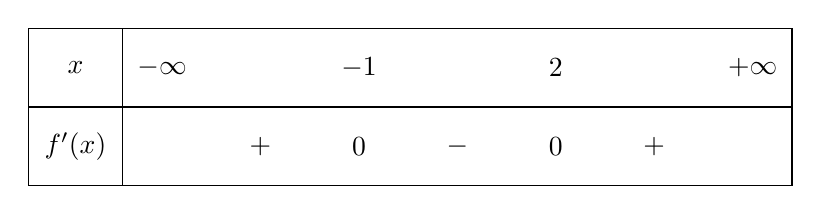
\begin{tikzpicture}[>=stealth]
    \tkzTabInit[nocadre=false,lgt=1.2,espcl=2.5]
    {$x$ / 1, $f'(x)$ / 1}
    {$-\infty$, $-1$, $2$, $+\infty$}
    \tkzTabLine{ , +, 0, -, 0, + }
\end{tikzpicture}
\end{center}
Hàm số đã cho đạt cực đại tại}{%
\begin{tasks}(4)
\task \( x = -2 \)
\task \( x = 2 \)
\task \( x = 1 \)
\task \( x = -1 \)
\end{tasks}
}

% ====== CÂU 16 ======
\questionLinesManual{5}{16}{Cho hàm \( f(x) \) liên tục trên \( \mathbb{R} \) có bảng xét dấu như sau:
\begin{center}
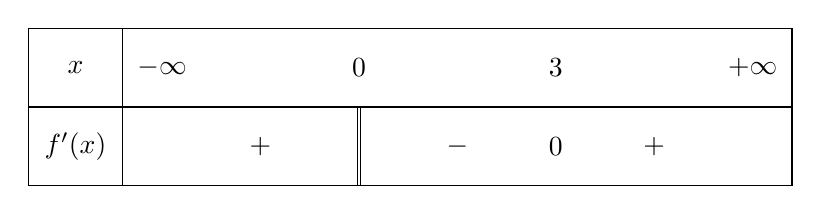
\begin{tikzpicture}[>=stealth]
    \tkzTabInit[nocadre=false,lgt=1.2,espcl=2.5]
    {$x$ / 1, $f'(x)$ / 1}
    {$-\infty$, $0$, $3$, $+\infty$}
    \tkzTabLine{ , +, d, -, 0, + }
\end{tikzpicture}
\end{center}
Hàm số có bao nhiêu điểm cực trị}{%
\begin{tasks}(4)
\task 3
\task 1
\task 0
\task 2
\end{tasks}
}

% ====== CÂU 17 ======
\questionLinesManual{5}{17}{Cho hàm số \( f(x) \) có bảng biến thiên như sau:
\begin{center}
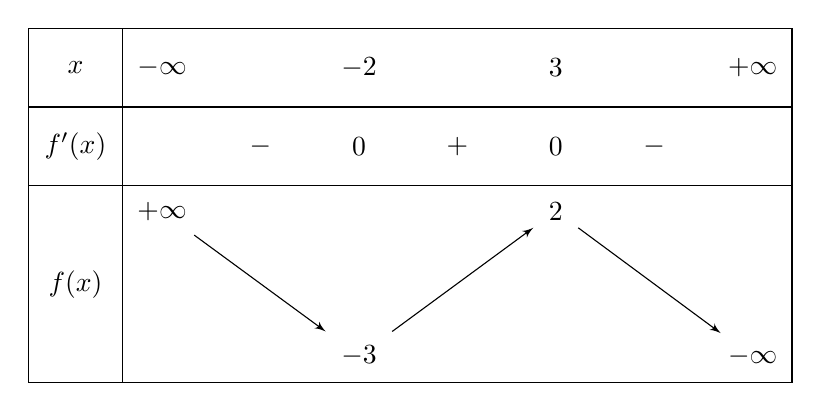
\begin{tikzpicture}[>=stealth]
    \tkzTabInit[nocadre=false,lgt=1.2,espcl=2.5]
    {$x$ / 1, $f'(x)$ / 1, $f(x)$ / 2.5}
    {$-\infty$, $-2$, $3$, $+\infty$}
    \tkzTabLine{ , -, 0, +, 0, - }
    \tkzTabVar{+/$+\infty$, -/$-3$, +/$2$,-/$-\infty$}
\end{tikzpicture}
\end{center}
Giá trị cực đại của hàm số đã cho bằng}{%
\begin{tasks}(4)
\task 3
\task 2
\task $-2$
\task $-3$
\end{tasks}
}

% ====== CÂU 18 ======
\questionLinesManual{5}{18}{Cho hàm số \( f(x) \) có bảng biến thiên như sau:
\begin{center}
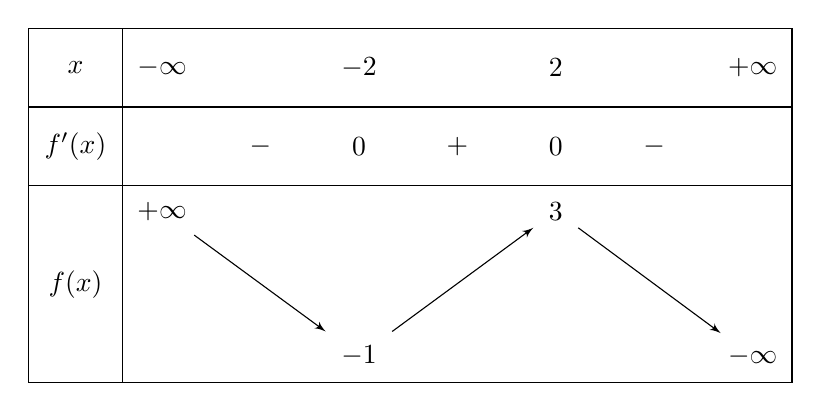
\begin{tikzpicture}[>=stealth]
    \tkzTabInit[nocadre=false,lgt=1.2,espcl=2.5]
    {$x$ / 1, $f'(x)$ / 1, $f(x)$ / 2.5}
    {$-\infty$, $-2$, $2$, $+\infty$}
    \tkzTabLine{ , -, 0, +, 0, - }
    \tkzTabVar{+/$+\infty$, -/$-1$, +/$3$,-/$-\infty$}
\end{tikzpicture}
\end{center}
Giá trị cực tiểu của hàm số đã cho bằng}{%
\begin{tasks}(4)
\task 2
\task $-2$
\task 3
\task $-1$
\end{tasks}
}

% ====== CÂU 19 ======
\questionLinesManual{5}{19}{Cho hàm số \( f(x) \) có bảng biến thiên như sau:
\begin{center}
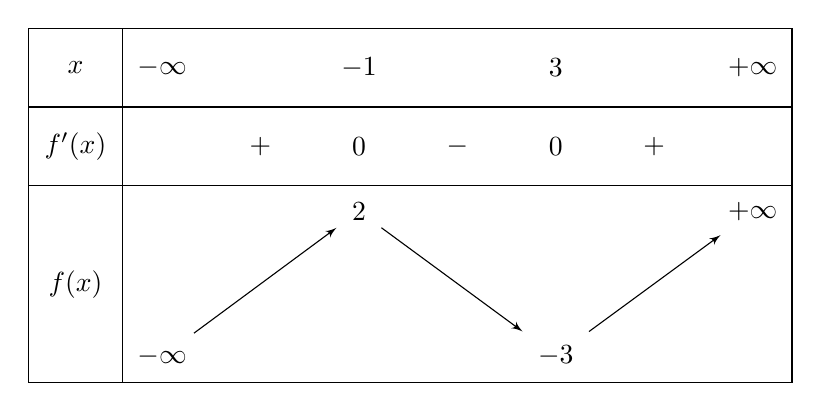
\begin{tikzpicture}[>=stealth]
    \tkzTabInit[nocadre=false,lgt=1.2,espcl=2.5]
    {$x$ / 1, $f'(x)$ / 1, $f(x)$ / 2.5}
    {$-\infty$, $-1$, $3$, $+\infty$}
    \tkzTabLine{ , +, 0, -, 0, + }
    \tkzTabVar{-/$-\infty$, +/$2$, -/$-3$,+/$+\infty$}
\end{tikzpicture}
\end{center}
Giá trị cực đại của hàm số đã cho bằng}{%
\begin{tasks}(4)
\task 3
\task $-3$
\task $-1$
\task 2
\end{tasks}
}

% ====== CÂU 20 ======
\questionLinesManual{5}{20}{Cho hàm số \( y = f(x) \) có bảng biến thiên như sau:
\begin{center}
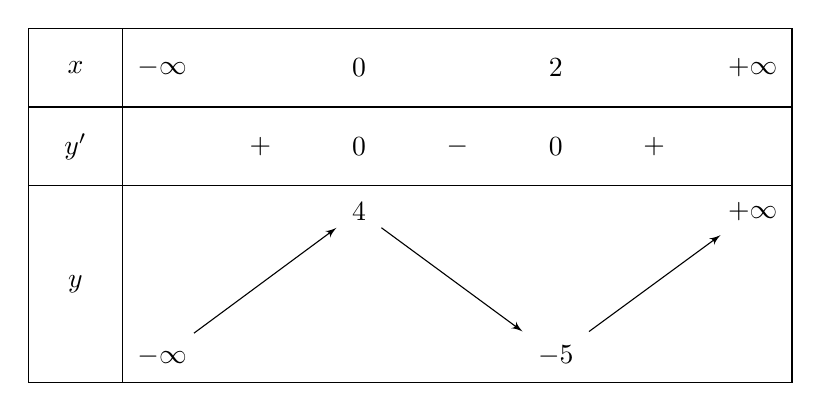
\begin{tikzpicture}[>=stealth]
    \tkzTabInit[nocadre=false,lgt=1.2,espcl=2.5]
    {$x$ / 1, $y'$ / 1, $y$ / 2.5}
    {$-\infty$, $0$, $2$, $+\infty$}
    \tkzTabLine{ , +, 0, -, 0, + }
   \tkzTabVar{-/$-\infty$, +/$4$, -/$-5$,+/$+\infty$}
\end{tikzpicture}
\end{center}
Mệnh đề nào dưới đây đúng?}{%
\begin{tasks}(2)
\task Hàm số đạt cực tiểu tại $x = -5$
\task Hàm số có bốn điểm cực trị
\task Hàm số đạt cực tiểu tại $x = 2$
\task Hàm số không có cực đại
\end{tasks}
}

% ====== CÂU 21 ======
\questionLinesManual{5}{21}{Cho hàm số \( y = f(x) \) có bảng biến thiên như sau:
\begin{center}
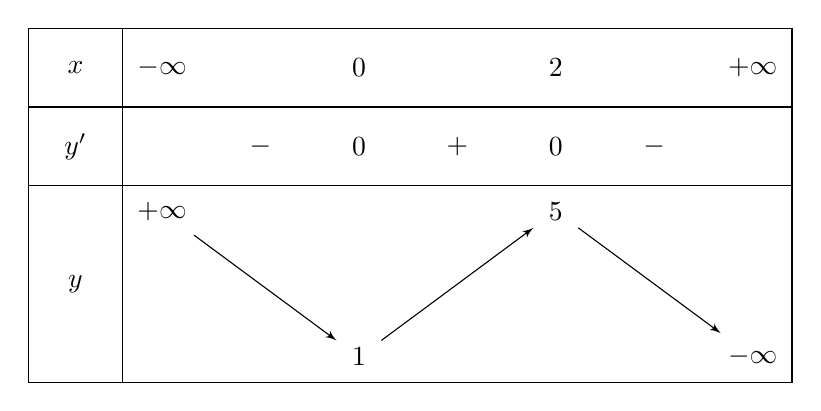
\begin{tikzpicture}[>=stealth]
    \tkzTabInit[nocadre=false,lgt=1.2,espcl=2.5]
    {$x$ / 1, $y'$ / 1, $y$ / 2.5}
    {$-\infty$, $0$, $2$, $+\infty$}
    \tkzTabLine{ , -, 0, +, 0, - }
    \tkzTabVar{+/$+\infty$, -/$1$, +/$5$,-/$-\infty$}
\end{tikzpicture}
\end{center}
Giá trị cực đại của hàm số đã cho bằng}{%
\begin{tasks}(4)
\task 5
\task 2
\task 0
\task 1
\end{tasks}
}

% ====== CÂU 22 ======
\questionLinesManual{5}{22}{Cho hàm số \( y = f(x) \) có bảng biến thiên như sau:
\begin{center}
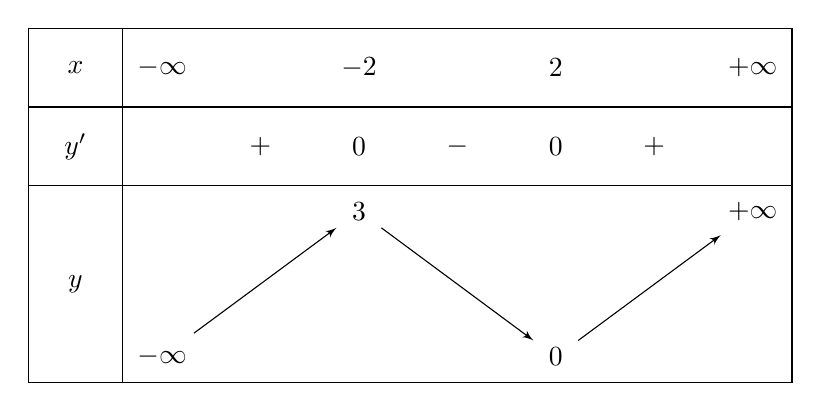
\begin{tikzpicture}[>=stealth]
    \tkzTabInit[nocadre=false,lgt=1.2,espcl=2.5]
    {$x$ / 1, $y'$ / 1, $y$ / 2.5}
    {$-\infty$, $-2$, $2$, $+\infty$}
    \tkzTabLine{ , +, 0, -, 0, + }
    \tkzTabVar{-/$-\infty$, +/$3$, -/$0$,+/$+\infty$}
\end{tikzpicture}
\end{center}
Tìm giá trị cực đại \( y_{CD} \) và giá trị cực tiểu \( y_{CT} \) của hàm số đã cho.}{%
\begin{tasks}(2)
\task \( y_{CD} = 2 \) và \( y_{CT} = 0 \)
\task \( y_{CD} = 3 \) và \( y_{CT} = 0 \)
\task \( y_{CD} = 3 \) và \( y_{CT} = -2 \)
\task \( y_{CD} = -2 \) và \( y_{CT} = 2 \)
\end{tasks}
}

% ====== CÂU 23 ======
\questionLinesManual{5}{23}{Cho hàm số \( f(x) \) liên tục trên \( \mathbb{R} \) có bảng xét dấu như sau:
\begin{center}
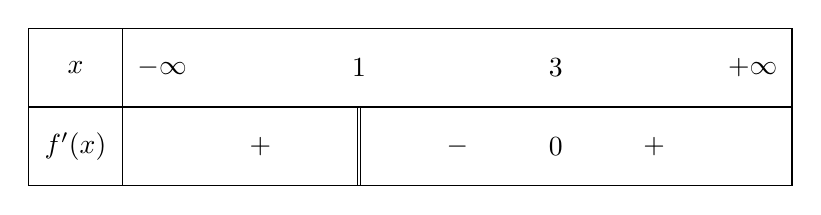
\begin{tikzpicture}[>=stealth]
    \tkzTabInit[nocadre=false,lgt=1.2,espcl=2.5]
    {$x$ / 1, $f'(x)$ / 1}
    {$-\infty$, $1$, $3$, $+\infty$}
    \tkzTabLine{ , +, d, -, 0, + }
\end{tikzpicture}
\end{center}
Hàm số có bao nhiêu điểm cực trị:}{%
\begin{tasks}(4)
\task 0
\task 1
\task 2
\task 3
\end{tasks}
}

% ====== CÂU 24 ======
\questionLinesManual{5}{24}{Cho hàm số \( f(x) \) xác đinh trên \(\mathbb{R} \setminus \{3\}\) có bảng xét dấu như sau:
\begin{center}
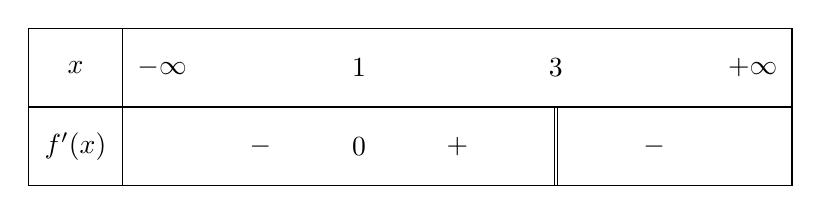
\begin{tikzpicture}[>=stealth]
    \tkzTabInit[nocadre=false,lgt=1.2,espcl=2.5]
    {$x$ / 1, $f'(x)$ / 1}
    {$-\infty$, $1$, $3$, $+\infty$}
    \tkzTabLine{ , -, 0, +, d, - }
\end{tikzpicture}
\end{center}
Hàm số có bao nhiêu điểm cực đại}{%
\begin{tasks}(4)
\task 0
\task 1
\task 2
\task 3
\end{tasks}
}

% ====== CÂU 25 ======
\questionLinesManual{5}{25}{Cho hàm số \( y = f(x) \) xác định trên \(\mathbb{R} \setminus \{1\}\) có bảng xét dấu như sau:
\begin{center}
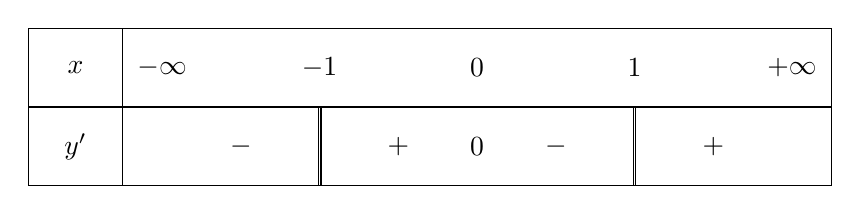
\begin{tikzpicture}[>=stealth]
    \tkzTabInit[nocadre=false,lgt=1.2,espcl=2]
    {$x$ / 1, $y'$ / 1}
    {$-\infty$, $-1$, $0$, $1$, $+\infty$}
    \tkzTabLine{ , -, d, +, 0, -, d, + }
\end{tikzpicture}
\end{center}
Hàm số có bao nhiêu điểm cực trị}{%
\begin{tasks}(4)
\task 0
\task 1
\task 2
\task 3
\end{tasks}
}
% ====== CÂU 26 ======
\questionLinesManual{5}{26}{Cho hàm số \( f(x) \) có bảng biến thiên như sau:
\begin{center}
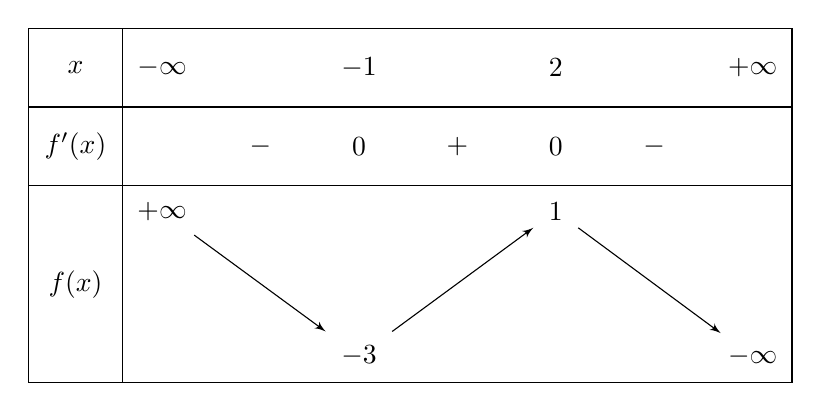
\begin{tikzpicture}[>=stealth]
    \tkzTabInit[nocadre=false,lgt=1.2,espcl=2.5]
    {$x$ / 1, $f'(x)$ / 1, $f(x)$ / 2.5}
    {$-\infty$, $-1$, $2$, $+\infty$}
    \tkzTabLine{ , -, 0, +, 0, - }
    \tkzTabVar{+/$+\infty$, -/$-3$, +/$1$,-/$-\infty$}
\end{tikzpicture}
\end{center}
Hàm số đã cho đạt cực tiểu tại}{%
\begin{tasks}(4)
\task $x = -1$
\task $x = -3$
\task $x = 2$
\task $x = 1$
\end{tasks}
}

% ====== CÂU 27 ======
\questionLinesManual{5}{27}{Cho hàm số \( y = f(x) \) có bảng biến thiên như sau:
\begin{center}
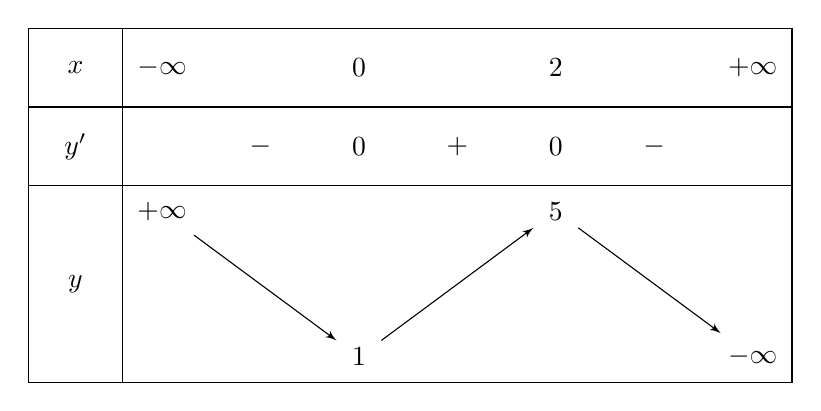
\begin{tikzpicture}[>=stealth]
    \tkzTabInit[nocadre=false,lgt=1.2,espcl=2.5]
    {$x$ / 1, $y'$ / 1, $y$ / 2.5}
    {$-\infty$, $0$, $2$, $+\infty$}
    \tkzTabLine{ , -, 0, +, 0, - }
    \tkzTabVar{+/$+\infty$, -/$1$, +/$5$,-/$-\infty$}
\end{tikzpicture}
\end{center}
Hàm số đạt cực đại tại điểm}{%
\begin{tasks}(4)
\task $x = 1$
\task $x = 0$
\task $x = 5$
\task $x = 2$
\end{tasks}
}

% ====== CÂU 28 ======
\questionLinesManual{5}{28}{Cho hàm số \( f(x) \) có bảng biến thiên như sau:
\begin{center}
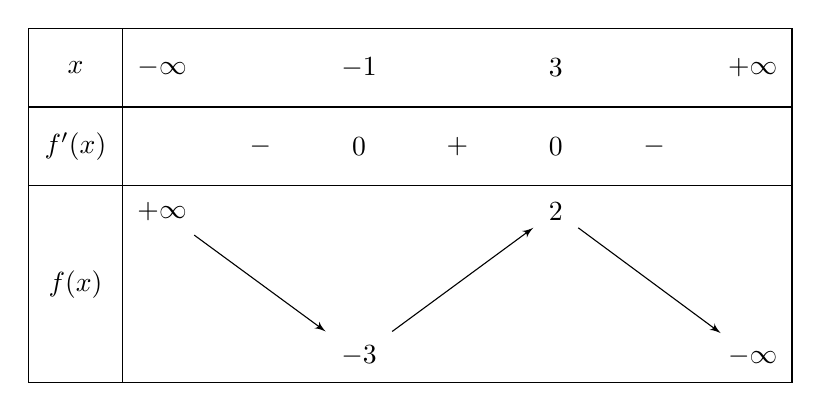
\begin{tikzpicture}[>=stealth]
    \tkzTabInit[nocadre=false,lgt=1.2,espcl=2.5]
    {$x$ / 1, $f'(x)$ / 1, $f(x)$ / 2.5}
    {$-\infty$, $-1$, $3$, $+\infty$}
    \tkzTabLine{ , -, 0, +, 0, - }
    \tkzTabVar{+/$+\infty$, -/$-3$, +/$2$,-/$-\infty$}
\end{tikzpicture}
\end{center}
Điểm cực đại của hàm số đã cho là}{%
\begin{tasks}(4)
\task $x = 3$
\task $x = -1$
\task $x = 2$
\task $x = -3$
\end{tasks}
}

% ====== CÂU 29 ======
\questionLinesManual{5}{29}{Cho hàm số \( f(x) \) có bảng biến thiên như sau:
\begin{center}
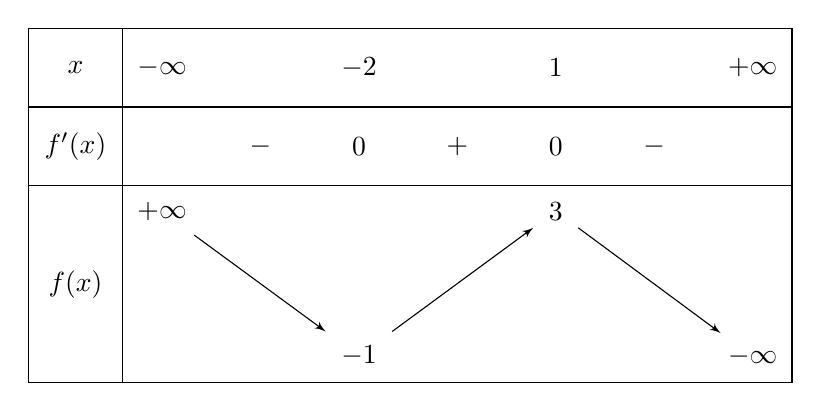
\begin{tikzpicture}[>=stealth]
    \tkzTabInit[nocadre=false,lgt=1.2,espcl=2.5]
    {$x$ / 1, $f'(x)$ / 1, $f(x)$ / 2.5}
    {$-\infty$, $-2$, $1$, $+\infty$}
    \tkzTabLine{ , -, 0, +, 0, - }
    \tkzTabVar{+/$+\infty$, -/$-1$, +/$3$,-/$-\infty$}
\end{tikzpicture}
\end{center}
Điểm cực đại của hàm số đã cho là}{%
\begin{tasks}(4)
\task $x = 3$
\task $x = -1$
\task $x = 1$
\task $x = -2$
\end{tasks}
}

% ====== CÂU 30 ======
\questionLinesManual{5}{30}{Cho hàm số \( f(x) \) có bảng biến thiên như sau:
\begin{center}
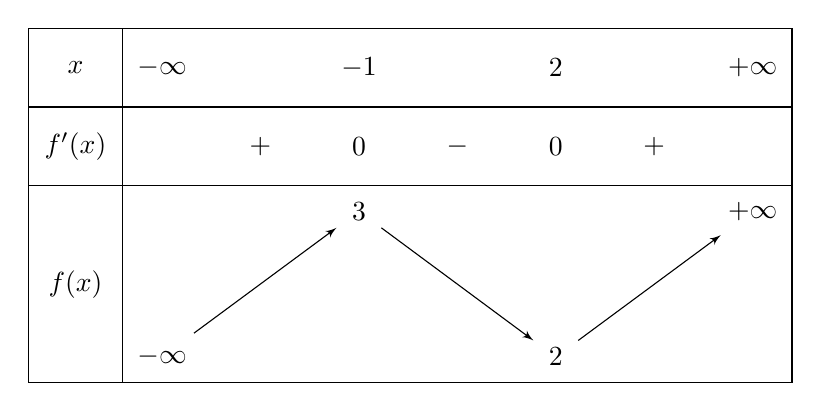
\begin{tikzpicture}[>=stealth]
    \tkzTabInit[nocadre=false,lgt=1.2,espcl=2.5]
    {$x$ / 1, $f'(x)$ / 1, $f(x)$ / 2.5}
    {$-\infty$, $-1$, $2$, $+\infty$}
    \tkzTabLine{ , +, 0, -, 0, + }
    
    \tkzTabVar{-/$-\infty$, +/$3$, -/$2$,+/$+\infty$}
\end{tikzpicture}
\end{center}
Điểm cực đại của hàm số đã cho là}{%
\begin{tasks}(4)
\task $x = 3$
\task $x = 2$
\task $x = -2$
\task $x = -1$
\end{tasks}
}

% ====== CÂU 31 ======
\questionLinesManual{5}{31}{Cho hàm số \( f(x) \) có bảng biến thiên như sau:
\begin{center}
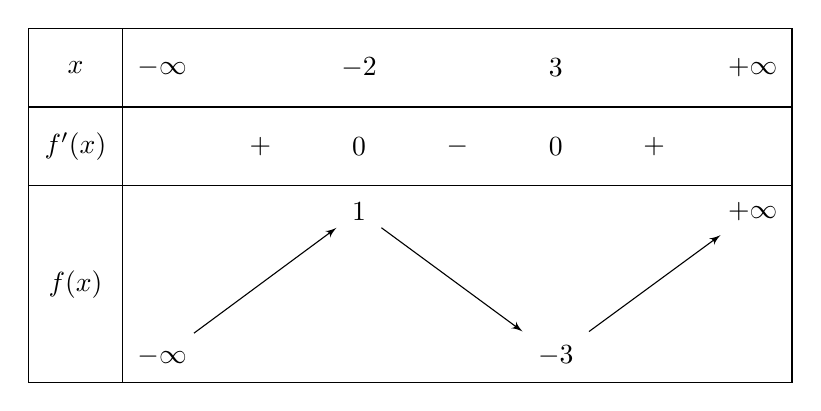
\begin{tikzpicture}[>=stealth]
    \tkzTabInit[nocadre=false,lgt=1.2,espcl=2.5]
    {$x$ / 1, $f'(x)$ / 1, $f(x)$ / 2.5}
    {$-\infty$, $-2$, $3$, $+\infty$}
    \tkzTabLine{ , +, 0, -, 0, + }
   \tkzTabVar{-/$-\infty$, +/$1$, -/$-3$,+/$+\infty$}
\end{tikzpicture}
\end{center}
Điểm cực đại của hàm số đã cho là}{%
\begin{tasks}(4)
\task $x = -2$
\task $x = -3$
\task $x = 1$
\task $x = 3$
\end{tasks}
}

% ====== CÂU 32 ======
\questionLinesManual{5}{32}{Cho hàm số \( y = f(x) \) có đồ thị như hình vẽ. Điểm cực tiểu của đồ thị hàm số đã cho là
\begin{center}
\begin{tikzpicture}[>=latex, scale=0.8]
    % Hệ trục tọa độ
    \draw[->] (-2.5,0) -- (3.5,0) node[below] {$x$};
    \draw[->] (0,-5) -- (0,2) node[right] {$y$};
    \node[above left] at (0,0) {$O$};
    
    % Đánh dấu các điểm
    \node[above] at (-1,0) {$-1$};
    \node[above] at (1,0) {$1$};
    \node[above right] at (2,0) {$2$};
    \node[left] at (0,-4) {$-4$};
    \node[left] at (0,-2) {$-2$};
    
    % Vẽ đồ thị hàm số y = x^3 - 3x^2 - 4x + 6
    \draw[thick, color=black!80, samples=150, domain=-1.65:2.1] 
        plot (\x, {\x*\x*\x - 3*\x - 2});
    
    % Đường nét đứt
    \draw[dashed] (1,0) -- (1,-4) -- (0,-4);
\end{tikzpicture}
\end{center}}{%
\begin{tasks}(4)
\task $-1$
\task $1$
\task $(2; 0)$
\task $(1; -4)$
\end{tasks}
}

% ====== CÂU 33 ======
\questionLinesManual{5}{33}{Cho hàm số bậc ba \( y = f(x) \) có đồ thị như hình vẽ dưới đây
\begin{center}
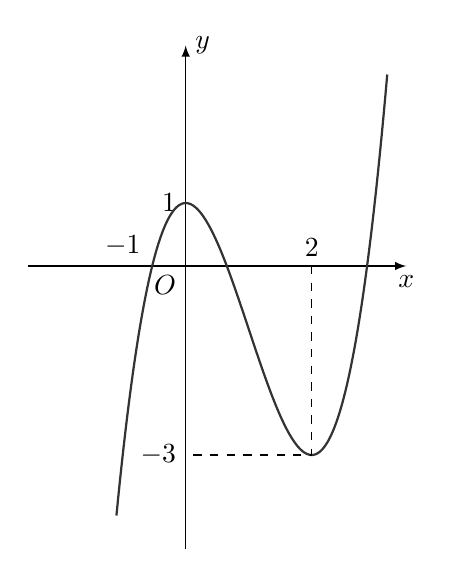
\begin{tikzpicture}[>=latex, scale=0.8]
    % Hệ trục tọa độ
    \draw[->] (-2.5,0) -- (3.5,0) node[below] {$x$};
    \draw[->] (0,-4.5) -- (0,3.5) node[right] {$y$};
    \node[below left] at (0,0) {$O$};
    
    % Đánh dấu các điểm
    \node[above] at (-1,0) {$-1$};
    \node[above] at (2,0) {$2$};
    \node[left] at (0,-3) {$-3$};
    \node[left] at (0,1) {$1$};
    
    % Vẽ đồ thị hàm bậc 3 y = x^3 - 3x^2 + 1
    \draw[thick, color=black!80, samples=150, domain=-1.1:3.2] 
        plot (\x, {\x*\x*\x - 3*\x*\x + 1});
    
    % Đường nét đứt
    \draw[dashed] (2,0) -- (2,-3) -- (0,-3);
\end{tikzpicture}
\end{center}
Giá trị cực tiểu của hàm số đã cho là}{%
\begin{tasks}(4)
\task $-3$
\task $2$
\task $1$
\task $0$
\end{tasks}
}

% ====== CÂU 34 ======
\questionLinesManual{5}{34}{Cho hàm đa thức \( y = f(x) \). Đồ thị hàm số \( y = f'(x) \) là đường cong như hình vẽ bên dưới. Hỏi hàm số \( y = f(x) \) có bao nhiêu điểm cực trị?
\begin{center}
\begin{tikzpicture}[>=latex, scale=0.8]
    % Hệ trục tọa độ
    \draw[->] (-4.5,0) -- (4.5,0) node[below] {$x$};
    \draw[->] (0,-3.5) -- (0,3.5) node[right] {$y$};
    \node[above left] at (0,0) {$O$};
    
    % Đánh dấu các điểm trên trục Ox
    \node[below] at (-2,0) {$-2$};
    \node[below] at (1,0) {$1$};
    \node[below] at (2,0) {$2$};
    
    % Vẽ đồ thị f'(x) (parabol bậc 3)
    \draw[thick, color=black!80, samples=150, domain=-1.2:3.2] 
       plot (\x, {-\x*\x*\x + 3*\x*\x - 1});
    \draw[dashed] (2,0) -- (2,3) -- (0,3);
    \node[right] at (3.5,2.5) {$y = f'(x)$};
\end{tikzpicture}
\end{center}}{%
\begin{tasks}(4)
\task 3
\task 1
\task 2
\task 0
\end{tasks}
}

% ====== CÂU 35 ======
\questionLinesManual{5}{35}{Cho hàm số \( y = f(x) \) có đồ thị như hình vẽ
\begin{center}
\begin{tikzpicture}[>=latex, scale=0.8]
    % Hệ trục tọa độ
    \draw[->] (-3.5,0) -- (3.5,0) node[below] {$x$};
    \draw[->] (0,-3.5) -- (0,3.5) node[right] {$y$};
    \node[above left] at (0,0) {$O$};
    
    % Đánh dấu các điểm trên trục
    \node[below] at (-1,0) {$-1$};
    \node[below] at (1,0) {$1$};
    \node[right] at (0,-2) {$-2$};
    \node[left] at (0,2) {$2$};
    
    % Vẽ đồ thị hàm số bậc 3 y = x^3 - 3x
    \draw[thick, color=black!80, samples=150, domain=-3:-0.3] 
       plot (\x, {(\x*\x + 1)/\x});
    \draw[thick, color=black!80, samples=150, domain=0.3:3] 
       plot (\x, {(\x*\x + 1)/\x});
    % Đường nét đứt
    \draw[dashed] (-1,0) -- (-1,-2) -- (0,-2);
    \draw[dashed] (1,0) -- (1,2)-- (0,2);
\end{tikzpicture}
\end{center}
Giá trị cực tiểu của hàm số đã cho là}{%
\begin{tasks}(4)
\task 1
\task $-1$
\task $-2$
\task 2
\end{tasks}
}

% ====== CÂU 36 ======
\questionLinesManual{5}{36}{Cho hàm số \( y = f(x) \) liên tục trên \( \mathbb{R} \) và có đồ thị như hình dưới đây.
\begin{center}
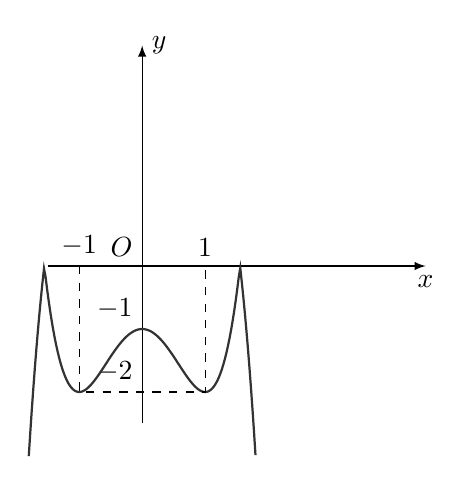
\begin{tikzpicture}[>=latex, scale=0.8]
    % Hệ trục tọa độ
    \draw[->] (-1.5,0) -- (4.5,0) node[below] {$x$};
    \draw[->] (0,-2.5) -- (0,3.5) node[right] {$y$};
    \node[above left] at (0,0) {$O$};
    
    % Đánh dấu các điểm trên trục
    \node[above] at (1,0) {$1$};
    \node[above] at (-1,0) {$-1$};
    \node[above left] at (0,-1) {$-1$};
    \node[above left] at (0,-2) {$-2$};
    
    % Vẽ đồ thị hàm bậc 4
    \draw[thick, color=black!80, samples=150, domain=-1.8:1.8] 
       plot (\x, {-abs(\x*\x*\x*\x - 2*\x*\x - 1)});
    % Đường nét đứt
    \draw[dashed] (-1,0) -- (-1,-2) -- (1,-2) -- (1,0);
\end{tikzpicture}
\end{center}
Hàm số đã cho có bao nhiêu điểm cực đại?}{%
\begin{tasks}(4)
\task 2
\task 3
\task 1
\task 5
\end{tasks}
}

% ====== CÂU 37 ======
\questionLinesManual{5}{37}{Cho hàm số \( y = f(x) \) có đồ thị như hình vẽ bên dưới. Điểm cực đại của đồ thị hàm số đã cho là:
\begin{center}
\begin{tikzpicture}[>=latex, scale=0.8]
    % Hệ trục tọa độ
    \draw[->] (-5,0) -- (3.5,0) node[below] {$x$};
    \draw[->] (0,-5) -- (0,3.5) node[right] {$y$};
    \node[below right] at (0,0) {$O$};
    
    % Đánh dấu các điểm
    \node[below] at (-3,0) {$-3$};
    \node[below] at (-1,0) {$-1$};
    \node[below] at (-2,0) {$-2$};
    \node[right] at (0,-3) {$-3$};
    \node[right] at (0,1) {$1$};
    
    % Vẽ đồ thị hàm bậc 3
    \draw[thick, color=black!80, samples=150, domain=-5:-2.2] 
        plot (\x, {(\x*\x + 3*\x + 3)/(\x + 2)});
    \draw[thick, color=black!80, samples=150, domain=-1.8:1.5] 
        plot (\x, {(\x*\x + 3*\x + 3)/(\x + 2)});
     \draw[thick, color=black!80, samples=150, domain=-5:1.7] 
       plot (\x, {\x + 1});   
    % Đường nét đứt
    \draw[dashed] (-3,0) -- (-3,-3) -- (0,-3);
    \draw[dashed] (-1,0) -- (-1,1) -- (0,1);
    \draw[-] (-2,3) -- (-2, -5);

\end{tikzpicture}
\end{center}}{%
\begin{tasks}(4)
\task $M(-3; -3)$
\task $x = -1$
\task $N(-1; 1)$
\task $x = -3$
\end{tasks}
}

% ====== CÂU 38 ======
\questionLinesManual{5}{38}{Cho hàm số có đồ thị như hình vẽ bên. Số điểm cực trị của hàm số đã cho là:
\begin{center}
\begin{tikzpicture}[>=latex, scale=0.8]
    % Hệ trục tọa độ
    \draw[->] (-3.5,0) -- (3.5,0) node[below] {$x$};
    \draw[->] (0,-2.5) -- (0,3.5) node[right] {$y$};
    \node[above left] at (0,0) {$O$};
    
    
    % Vẽ đồ thị hàm bậc 3
    \draw[thick, color=black!80, samples=150, domain=-2.3:2.3] 
       plot (\x, {-0.5*\x*\x*\x*\x +2*\x*\x+2 });
\end{tikzpicture}
\end{center}}{%
\begin{tasks}(4)
\task 3
\task 1
\task 2
\task 0
\end{tasks}
}

% ====== CÂU 39 ======
\questionLinesManual{5}{39}{Cho hàm số \( y = ax^4 + bx^2 + c \) (\( a, b, c \in \mathbb{R} \)) có đồ thị như hình vẽ bên.
\begin{center}
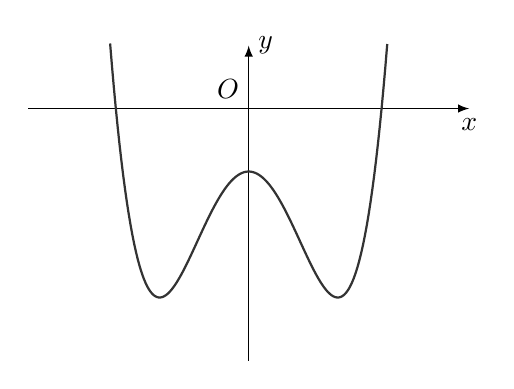
\begin{tikzpicture}[>=latex, scale=0.8]
    % Hệ trục tọa độ
    \draw[->] (-3.5,0) -- (3.5,0) node[below] {$x$};
    \draw[->] (0,-4) -- (0,1) node[right] {$y$};
    \node[above left] at (0,0) {$O$};
    
    
    % Vẽ đồ thị hàm bậc 4 trùng phương y = x^4 - 4x^2
    \draw[thick, color=black!80, samples=150, domain=-2.2:2.2] 
        plot (\x, {0.5*\x*\x*\x*\x - 2*\x*\x - 1});
    
\end{tikzpicture}
\end{center}
Số điểm cực trị của hàm số đã cho là}{%
\begin{tasks}(4)
\task 3
\task 0
\task 1
\task 2
\end{tasks}
}

% ====== CÂU 40 ======
\questionLinesManual{5}{40}{Cho hàm số \( y = ax^3 + bx^2 + cx + d \) (\( a, b, c, d \in \mathbb{R} \)) có đồ thị như hình vẽ bên. Số điểm cực trị của hàm số này là
\begin{center}
\begin{tikzpicture}[>=latex, scale=0.8]
    % Hệ trục tọa độ
    \draw[->] (-3.5,0) -- (3.5,0) node[below] {$x$};
    \draw[->] (0,-3.5) -- (0,3.5) node[right] {$y$};
    \node[above left] at (0,0) {$O$};
    
    
    % Vẽ đồ thị hàm bậc 3 y = x^3 - 3x
    \draw[thick, color=black!80, samples=150, domain=-2.1:2.1] 
        plot (\x, {\x*\x*\x - 3*\x});
    
\end{tikzpicture}
\end{center}}{%
\begin{tasks}(4)
\task 3
\task 2
\task 0
\task 1
\end{tasks}
}

% ====== CÂU 41 ======
\questionLinesManual{5}{41}{Cho hàm số \( y = ax^3 + bx^2 + cx + d \) (\( a, b, c, d \in \mathbb{R} \)) có đồ thị như hình vẽ bên. Số điểm cực trị của hàm số đã cho là
\begin{center}
\begin{tikzpicture}[>=latex, scale=0.8]
    % Hệ trục tọa độ
    \draw[->] (-3.5,0) -- (3.5,0) node[below] {$x$};
    \draw[->] (0,-3.5) -- (0,3.5) node[right] {$y$};
    \node[above left] at (0,0) {$O$};
    
    
    % Vẽ đồ thị hàm bậc 3 y = -x^3 + 3x
    \draw[thick, color=black!80, samples=150, domain=-2.1:2.1] 
        plot (\x, {-\x*\x*\x + 3*\x});
    
    
\end{tikzpicture}
\end{center}}{%
\begin{tasks}(4)
\task 2
\task 0
\task 3
\task 1
\end{tasks}
}

% ====== CÂU 42 ======
\questionLinesManual{8}{42}{Đồ thị hàm số \( y = x^3 - 6x^2 + 9x - 1 \) có toạ độ điểm cực đại là}{%
\begin{tasks}(4)
\task \( (3; 0) \)
\task \( (3; 1) \)
\task \( (1; 4) \)
\task \( (1; 3) \)
\end{tasks}
}

% ====== CÂU 43 ======
\questionLinesManual{8}{43}{Cho hàm số \( y = x^3 - 3x^2 + 2 \). Mệnh đề nào dưới đây đúng?}{%
\begin{tasks}(2)
\task Hàm số đạt cực tiểu tại điểm \( x = 0 \)
\task Hàm số đạt cực đại tại điểm \( M(0; 2) \)
\task Hàm số đạt cực đại tại điểm \( x = 0 \)
\task Hàm số đạt cực đại tại điểm \( x = 2 \)
\end{tasks}
}

% ====== CÂU 44 ======
\questionLinesManual{8}{44}{Số điểm cực tiểu của hàm số \( f(x) = x^4 - x^2 + 2 \) là}{%
\begin{tasks}(4)
\task 2
\task 4
\task 1
\task 3
\end{tasks}
}

% ====== CÂU 45 ======
\questionLinesManual{8}{45}{Tìm giá trị cực đại \( y_{CD} \) của hàm số \( y = x^3 - 3x + 2 \).}{%
\begin{tasks}(4)
\task \( y_{CD} = -1 \)
\task \( y_{CD} = 4 \)
\task \( y_{CD} = 1 \)
\task \( y_{CD} = 0 \)
\end{tasks}
}

% ====== CÂU 46 ======
\questionLinesManual{8}{46}{Hàm số \( y = \dfrac{2x + 3}{x + 1} \) có bao nhiêu điểm cực trị?}{%
\begin{tasks}(4)
\task 1
\task 3
\task 0
\task 2
\end{tasks}
}

% ====== CÂU 47 ======
\questionLinesManual{8}{47}{Cho hàm số \( y = \dfrac{x^2 + 3}{x + 1} \). Mệnh đề nào dưới đây đúng?}{%
\begin{tasks}(2)
\task Cực tiểu của hàm số bằng \(-3\)
\task Cực tiểu của hàm số bằng \(1\)
\task Cực tiểu của hàm số bằng \(-6\)
\task Cực tiểu của hàm số bằng \(2\)
\end{tasks}
}

% ====== CÂU 48 ======
\questionLinesManual{8}{48}{Điểm cực đại của đồ thị hàm số \( y = x^3 - 6x^2 + 9x \) có tổng hoành độ và tung độ bằng}{%
\begin{tasks}(4)
\task 5
\task 1
\task 3
\task -1
\end{tasks}
}

% ====== CÂU 49 ======
\questionLinesManual{8}{49}{Tìm giá trị cực đại của hàm số \( y = x^3 - 3x^2 - 2 \).}{%
\begin{tasks}(4)
\task $-2$
\task $0$
\task $2$
\task $1$
\end{tasks}
}

% ====== CÂU 50 ======
\questionLinesManual{8}{50}{Điểm cực đại của đồ thị hàm số \( y = -x^3 + 3x + 1 \) là:}{%
\begin{tasks}(4)
\task $M(-1; -1)$
\task $N(0; 1)$
\task $P(2; -1)$
\task $Q(1; 3)$
\end{tasks}
}

% ====== CÂU 51 ======
\questionLinesManual{8}{51}{Hàm số \( y = \dfrac{1}{3}x^3 + x^2 - 3x + 1 \) đạt cực tiểu tại điểm}{%
\begin{tasks}(4)
\task $x = -1$
\task $x = 1$
\task $x = -3$
\task $x = 3$
\end{tasks}
}

% ====== CÂU 52 ======
\questionLinesManual{8}{52}{Tìm số điểm cực trị của hàm số \( y = x^4 - 2x^2 \).}{%
\begin{tasks}(4)
\task $2$
\task $4$
\task $3$
\task $1$
\end{tasks}
}

% ====== CÂU 53 ======
\questionLinesManual{8}{53}{Điểm cực tiểu của đồ thị hàm số \( y = -x^3 + x^2 + 5x - 5 \) là}{%
\begin{tasks}(4)
\task $(-1; -8)$
\task $(0; -5)$
\task $\left(\dfrac{5}{3}; \dfrac{40}{27}\right)$
\task $(1; 0)$
\end{tasks}
}

% ====== CÂU 54 ======
\questionLinesManual{8}{54}{Tìm giá trị cực tiểu \( y_{CT} \) của hàm số \( y = -x^3 + 3x - 4 \).}{%
\begin{tasks}(4)
\task \( y_{CT} = -6 \)
\task \( y_{CT} = -1 \)
\task \( y_{CT} = -2 \)
\task \( y_{CT} = 1 \)
\end{tasks}
}

% ====== CÂU 55 ======
\questionLinesManual{8}{55}{Giá trị cực tiểu \( y_{CT} \) của hàm số \( y = x^3 - 3x^2 + 4 \) là:}{%
\begin{tasks}(4)
\task \( y_{CT} = 0 \)
\task \( y_{CT} = 3 \)
\task \( y_{CT} = 2 \)
\task \( y_{CT} = 4 \)
\end{tasks}
}

% ====== CÂU 56 ======
\questionLinesManual{8}{56}{Đồ thị hàm số \( y = x^4 - x^2 + 1 \) có bao nhiêu điểm cực trị có tung độ là số dương?}{%
\begin{tasks}(4)
\task 3
\task 1
\task 2
\task 0
\end{tasks}
}

% ====== CÂU 57 ======
\questionLinesManual{8}{57}{Hàm số nào dưới đây không có cực trị?}{%
\begin{tasks}(4)
\task \( y = \dfrac{2x + 1}{x - 3} \)
\task \( y = x^3 - x^2 - 3x + 2 \)
\task \( y = -x^3 + 3x^2 + 1 \)
\task \( y = x^3 - 3x^2 + 2 \)
\end{tasks}
}

% ====== CÂU 58 ======
\questionLinesManual{8}{58}{Hàm số \( y = \dfrac{x^2 + x + 4}{x + 1} \) có tất cả bao nhiêu cực trị?}{%
\begin{tasks}(4)
\task 2
\task 3
\task 1
\task 0
\end{tasks}
}

% ====== CÂU 59 ======
\questionLinesManual{8}{59}{Hàm số nào dưới đây không có cực trị?}{%
\begin{tasks}(4)
\task \( y = \dfrac{x^2 + 1}{x} \)
\task \( y = \dfrac{2x - 2}{x + 1} \)
\task \( y = x^2 - 2x + 1 \)
\task \( y = -x^3 + x + 1 \)
\end{tasks}
}

% ====== CÂU 60 ======
\questionLinesManual{8}{60}{Hàm số nào trong bốn hàm số được liệt kê dưới đây không có cực trị?}{%
\begin{tasks}(4)
\task \( y = \dfrac{2x - 3}{x + 2} \)
\task \( y = x^4 \)
\task \( y = -x^3 + x \)
\task \( y = |x + 2| \)
\end{tasks}
}

% ====== CÂU 61 ======
\questionLinesManual{8}{61}{Cho hàm số \( y = f(x) \) liên tục trên \( \mathbb{R} \) và có đạo hàm  
\( f'(x) = (x+1)^3(x-1)(x-2). \) 
Số điểm cực trị của hàm số đã cho là}{%
\begin{tasks}(4)
\task 1
\task 3
\task 2
\task 0
\end{tasks}
}

% ====== CÂU 62 ======
\questionLinesManual{8}{62}{Hàm số \( f(x) \) có đạo hàm  
\( f'(x) = x^2(x-1)(x-2)^3, \quad \forall x \in \mathbb{R}. \)  
Hàm số \( f(x) \) có bao nhiêu điểm cực đại?}{%
\begin{tasks}(4)
\task 2
\task 0
\task 3
\task 1
\end{tasks}
}

% ====== CÂU 63 ======
\questionLinesManual{5}{63}{Cho hàm số \( y = f(x) \) xác định trên \( \mathbb{R} \) và có đạo hàm  
\( f'(x) = x^{2024}(3-x), \quad \forall x \in \mathbb{R}. \) 
Hàm số đã cho có mấy điểm cực trị?}{%
\begin{tasks}(4)
\task 3
\task 0
\task 2
\task 1
\end{tasks}
}

% ====== CÂU 64 ======
\questionLinesManual{5}{64}{Cho hàm số \( f(x) \) có đạo hàm  
\( f'(x) = x^2(x+2)(x^2+x-2)(x-1)^4 \)
với mọi \( x \in \mathbb{R} \). Số điểm cực trị của hàm số đã cho là}{%
\begin{tasks}(4)
\task 3
\task 2
\task 1
\task 0
\end{tasks}
}

% ====== CÂU 65 ======
\questionLinesManual{5}{65}{Cho hàm số \( f(x) \) có đạo hàm  
\( f'(x) = x(x-1)(x-2)^2, \quad \forall x \in \mathbb{R}. \)  
Số điểm cực trị của hàm số đã cho là}{%
\begin{tasks}(4)
\task 5
\task 2
\task 1
\task 3
\end{tasks}
}

% ====== CÂU 66 ======
\questionLinesManual{5}{66}{Cho hàm số \( f(x) \) có đạo hàm \( f'(x) = x(x-1)(x+4)^3 \), \( \forall x \in \mathbb{R} \). Số điểm cực đại của hàm số đã cho là}{%
\begin{tasks}(4)
\task 3
\task 4
\task 2
\task 1
\end{tasks}
}

% ====== CÂU 67 ======
\questionLinesManual{5}{67}{Cho hàm số \( f(x) \) có đạo hàm \( f'(x) = x(x+1)(x-4)^3 \), \( \forall x \in \mathbb{R} \). Số điểm cực đại của hàm số đã cho là}{%
\begin{tasks}(4)
\task 2
\task 3
\task 4
\task 1
\end{tasks}
}

% ====== CÂU 68 ======
\questionLinesManual{5}{68}{Cho hàm số \( f(x) \) có \( f'(x) = x(x+1)(x-4)^3 \), \( \forall x \in \mathbb{R} \). Số điểm cực tiểu của hàm số đã cho là}{%
\begin{tasks}(4)
\task 4
\task 3
\task 1
\task 2
\end{tasks}
}

% ====== CÂU 69 ======
\questionLinesManual{5}{69}{Cho hàm số \( f(x) \) có đạo hàm \( f'(x) = x(x-1)(x+4)^3 \), \( \forall x \in \mathbb{R} \). Số điểm cực tiểu của hàm số đã cho là}{%
\begin{tasks}(4)
\task 2
\task 3
\task 4
\task 1
\end{tasks}
}

% ====== CÂU 70 ======
\questionLinesManual{5}{70}{Cho hàm số \( f(x) \) có đạo hàm \( f'(x) = x(x-1)(x+2)^3 \), \( \forall x \in \mathbb{R} \). Số điểm cực trị của hàm số đã cho là}{%
\begin{tasks}(4)
\task 1
\task 3
\task 2
\task 5
\end{tasks}
}

% ====== CÂU 71 ======
\questionLinesManual{5}{71}{Cho hàm số \( f(x) \) có đạo hàm \( f'(x) = x(x+2)^2 \), \( \forall x \in \mathbb{R} \). Số điểm cực trị của hàm số đã cho là}{%
\begin{tasks}(4)
\task 2
\task 1
\task 0
\task 3
\end{tasks}
}

% ====== CÂU 72 ======
\questionLinesManual{5}{72}{Cho hàm số \( f(x) \) có đạo hàm \( f'(x) = x(x-1)^2 \), \( \forall x \in \mathbb{R} \). Số điểm cực trị của hàm số đã cho là}{%
\begin{tasks}(4)
\task 2
\task 0
\task 1
\task 3
\end{tasks}
}

% ====== CÂU 73 ======
\questionLinesManual{5}{73}{Cho hàm số \( f(x) \) có đạo hàm \( f'(x) = x(x+1)^2 \), \( \forall x \in \mathbb{R} \). Số điểm cực trị của hàm số đã cho là}{%
\begin{tasks}(4)
\task 1
\task 2
\task 3
\task 0
\end{tasks}
}

% ====== CÂU 74 ======
\questionLinesManual{5}{74}{Cho hàm số \( y = f(x) \) có đạo hàm \( f'(x) = x(x-2)^2 \), \( \forall x \in \mathbb{R} \). Số điểm cực trị của hàm số đã cho là}{%
\begin{tasks}(4)
\task 0
\task 3
\task 2
\task 1
\end{tasks}
}

% ====== CÂU 75 ======
\questionLinesManual{5}{75}{Cho hàm số \( f(x) \) có đạo hàm  
\( f'(x) = x(1-x)^2 (3-x)^3 (x-2)^4 \)
với mọi \( x \in \mathbb{R} \). Điểm cực tiểu của hàm số đã cho là}{%
\begin{tasks}(4)
\task \( x = 2 \)
\task \( x = 3 \)
\task \( x = 0 \)
\task \( x = 1 \)
\end{tasks}
}

% ====== CÂU 76 ======
\questionLinesManual{5}{76}{Cho hàm số \( f(x) \) có đạo hàm \( f'(x) = x^3(x-1)(x-2) \), \( \forall x \in \mathbb{R} \). Số điểm cực trị của hàm số đã cho là}{%
\begin{tasks}(4)
\task 1
\task 3
\task 5
\task 2
\end{tasks}
}

% ====== CÂU 77 ======
\questionLinesManual{10}{77}{Hàm số \( y = f(x) \) có đạo hàm \( f'(x) = (x-1)(x-2)...(x-2019), \forall x \in \mathbb{R} \). Hàm số \( y = f(x) \) có tất cả bao nhiêu điểm cực tiểu?}{%
\begin{tasks}(4)
\task 1008
\task 1010
\task 1009
\task 1011
\end{tasks}
}

% ====== CÂU 78 ======
\questionLinesManual{5}{78}{Hàm số \( f(x) \) có đạo hàm \( f'(x) = x^2(x+1)(x-2)^3, \forall x \in \mathbb{R} \). Hỏi \( f(x) \) có bao nhiêu điểm cực đại?}{%
\begin{tasks}(4)
\task 2
\task 0
\task 1
\task 3
\end{tasks}
}

% ====== CÂU 79 ======
\questionLinesManual{5}{79}{Cho hàm số \( f(x) \) có đạo hàm là \( f'(x) = x(x-1)(x+2)^2 \forall x \in \mathbb{R} \). Số điểm cực trị của hàm số là?}{%
\begin{tasks}(4)
\task 5
\task 2
\task 1
\task 3
\end{tasks}
}

% ====== CÂU 80 ======
\questionLinesManual{5}{80}{Cho hàm số \( f(x) \) có đạo hàm  
\( f'(x) = (x-1)(x-2)^2(x-3)^3(x-4)^4, \forall x \in \mathbb{R} \). Số điểm cực trị của hàm số đã cho là}{%
\begin{tasks}(4)
\task 3
\task 5
\task 2
\task 4
\end{tasks}
}

% ====== CÂU 81 ======
\questionLinesManual{5}{81}{Cho hàm số \( f(x) \) có đạo hàm  
\( f'(x) = x(x-1)(x-2)^2, \forall x \in \mathbb{R} \). Số điểm cực trị của hàm số đã cho là}{%
\begin{tasks}(4)
\task 5
\task 2
\task 1
\task 3
\end{tasks}
}

% ====== CÂU 82 ======
\questionLinesManual{5}{82}{Cho hàm số \( y = f(x) \) có đạo hàm  
\( f'(x) = (x-2)(x^2-3)(x^4-9) \). Số điểm cực trị của hàm số \( y = f(x) \) là}{%
\begin{tasks}(4)
\task 3
\task 4
\task 2
\task 1
\end{tasks}
}

% ====== CÂU 83 ======
\questionLinesManual{8}{83}{Nếu hàm số \( f(x) \) có đạo hàm là  
\( f'(x) = x^2(x-2)(x^2-x-2)(x+1)^4 \) 
thì tổng các điểm cực trị của hàm số \( f(x) \) bằng}{%
\begin{tasks}(4)
\task $-1$
\task 2
\task 1
\task 0
\end{tasks}
}

% ====== CÂU 84 ======
\questionLinesManual{8}{84}{Cho hàm số \( y = f(x) \) có đạo hàm  
\( f'(x) = x(x^2+2x)^3(x^2-\sqrt{2}) \)  
với \( x \in \mathbb{R} \). Số điểm cực trị của hàm số là}{%
\begin{tasks}(4)
\task 4
\task 1
\task 2
\task 3
\end{tasks}
}

% ====== CÂU 85 ======
\questionLinesManual{5}{85}{Cho hàm số \( y = f(x) \) có đạo hàm trên \( \mathbb{R} \) và  
\( f'(x) = (x-1)(x-2)^2(x+3) \)  
Số điểm cực trị của hàm số đã cho là:}{%
\begin{tasks}(4)
\task 3
\task 1
\task 0
\task 2
\end{tasks}
}

% ====== CÂU 86 ======
\questionLinesManual{5}{86}{Cho hàm đa thức \( y = f(x) \). Đồ thị hàm số \( y = f'(x) \) là đường cong như hình vẽ bên dưới. Hỏi hàm số \( y = f(x) \) có bao nhiêu điểm cực trị?
\begin{center}
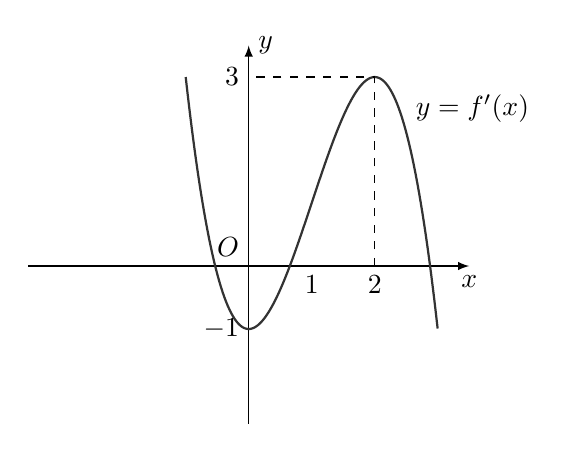
\begin{tikzpicture}[>=latex, scale=0.8]
    % Hệ trục tọa độ
    \draw[->] (-3.5,0) -- (3.5,0) node[below] {$x$};
    \draw[->] (0,-2.5) -- (0,3.5) node[right] {$y$};
    \node[above left] at (0,0) {$O$};
    
    % Đánh dấu các điểm
    \node[left] at (0,-1) {$-1$};
    \node[below] at (1,0) {$1$};
    \node[below] at (2,0) {$2$};
    \node[left] at (0,3) {$3$};
    
    % Vẽ đồ thị f'(x)
    \draw[thick, color=black!80, samples=150, domain=-1:3] 
       plot (\x, {-\x*\x*\x + 3*\x*\x - 1});
    \draw[dashed] (2,0) -- (2,3) -- (0,3);
    \node[right] at (2.5,2.5) {$y = f'(x)$};
\end{tikzpicture}
\end{center}}{%
\begin{tasks}(4)
\task 3
\task 1
\task 2
\task 0
\end{tasks}
}

% ====== CÂU 87 ======
\questionLinesManual{5}{87}{Cho hàm số \( y = f(x) \) có đạo hàm trên \( \mathbb{R} \). Biết hàm số \( y = f'(x) \) có đồ thị như hình vẽ. Phát biểu nào sau đây là đúng?
\begin{center}
\begin{tikzpicture}[>=latex, scale=0.8]
    % Hệ trục tọa độ
    \draw[->] (-3.5,0) -- (3.5,0) node[below] {$x$};
    \draw[->] (0,-2) -- (0,3.5) node[right] {$y$};
    \node[above left] at (0,0) {$O$};
    
    % Đánh dấu các điểm
    \node[below] at (-2,0) {$-2$};
    \node[below] at (1,0) {$1$};
    \node[right] at (0,2) {$2$};
    
    % Vẽ đồ thị f'(x) là parabol hướng xuống có nghiệm tại x = -2 và x = 1
    \draw[thick, color=black!80, samples=150, domain=-2.3:1.3] 
        plot (\x, {-(\x+2)*(\x-1)});
    
    \node[right] at (1.5,2) {$y = f'(x)$};
\end{tikzpicture}
\end{center}}{%
\begin{tasks}(1)
\task Hàm số \( y = f(x) \) đạt cực đại tại \( x_1 = -2 \) và đạt cực tiểu tại \( x_2 = 1 \).
\task Hàm số \( y = f(x) \) đạt cực tiểu tại hai điểm \( x_1 = -2 \) và \( x_2 = 1 \).
\task Hàm số \( y = f(x) \) đạt cực đại tại hai điểm \( x_1 = -2 \) và \( x_2 = 1 \).
\task Hàm số \( y = f(x) \) đạt cực tiểu tại \( x_1 = -2 \) và đạt cực đại tại \( x_2 = 1 \).
\end{tasks}
}

% ====== CÂU 88 (Đúng/Sai) ======
\questionTrueFalse{15}{88}{Biết rằng hàm số \( f(x) = 2x^3 + ax^2 - 6x + b \) ( \( a \) và \( b \) là hằng số thực) đạt cực trị bằng 4 tại \( x = 1 \).}{
    \textbf{a)} & Giá trị của \( a + b \) bằng 8.
    & \textcolor{amberorange}{$\bigcirc$} & \textcolor{amberorange}{$\bigcirc$} \\ \hline
    \textbf{b)} & Hàm số đạt cực đại tại \( x = 1 \).
    & \textcolor{amberorange}{$\bigcirc$} & \textcolor{amberorange}{$\bigcirc$} \\ \hline
    \textbf{c)} & \( x = -1 \) là một điểm cực trị của hàm số \( f(x) \).
    & \textcolor{amberorange}{$\bigcirc$} & \textcolor{amberorange}{$\bigcirc$} \\ \hline
    \textbf{d)} & Giá trị cực tiểu của hàm số \( f(x) \) bằng 12.
    & \textcolor{amberorange}{$\bigcirc$} & \textcolor{amberorange}{$\bigcirc$} \\
}

% ====== CÂU 89 (Đúng/Sai) ======
\questionTrueFalse{15}{89}{Cho hàm số \( f(x) \) xác định trên \( \mathbb{R} \) và đạo hàm \( f'(x) \) có đồ thị như hình bên. Sử dụng đồ thị của hàm số \( y = f'(x) \).
\begin{center}
\begin{tikzpicture}[>=latex, scale=0.8]
    % Hệ trục tọa độ
    \draw[->] (-1.5,0) -- (5.5,0) node[below] {$x$};
    \draw[->] (0,-2.5) -- (0,5) node[right] {$y$};
    \node[above left] at (0,0) {$O$};
    
    % Đánh dấu các điểm
    \node[below] at (4,0) {$4$};
    \node[below] at (2,0) {$2$};
    
    % Vẽ đồ thị f'(x) là parabol hướng lên có nghiệm tại x = 0 và x = 4
    \draw[thick, color=black!80, samples=150, domain=-0.5:4.5] 
        plot (\x, {-((\x)*( (\x)-4))});
    
    \node[right] at (3,3) {$y = f'(x)$};
\end{tikzpicture}
\end{center}}{
    \textbf{a)} & Hàm số \( f(x) \) nghịch biến trên các khoảng \( (-\infty; 0) \) và \( (4; +\infty) \).
    & \textcolor{amberorange}{$\bigcirc$} & \textcolor{amberorange}{$\bigcirc$} \\ \hline
    \textbf{b)} & Hàm số \( f(x) \) đồng biến trên khoảng \( (0; 4) \).
    & \textcolor{amberorange}{$\bigcirc$} & \textcolor{amberorange}{$\bigcirc$} \\ \hline
    \textbf{c)} & Hàm số \( f(x) \) đạt cực đại tại \( x = 0 \).
    & \textcolor{amberorange}{$\bigcirc$} & \textcolor{amberorange}{$\bigcirc$} \\ \hline
    \textbf{d)} & Hàm số \( f(x) \) đạt cực tiểu tại \( x = 4 \).
    & \textcolor{amberorange}{$\bigcirc$} & \textcolor{amberorange}{$\bigcirc$} \\
}

% ====== CÂU 90 (Đúng/Sai) ======
\questionTrueFalse{15}{90}{Cho hàm số \( f(x) \) có bảng biến thiên như sau:
\begin{center}
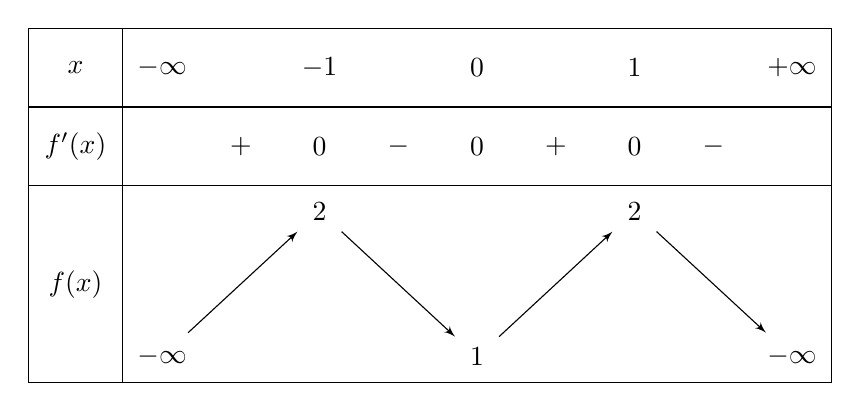
\begin{tikzpicture}[>=stealth]
    \tkzTabInit[nocadre=false,lgt=1.2,espcl=2]
    {$x$ / 1, $f'(x)$ / 1, $f(x)$ / 2.5}
    {$-\infty$, $-1$, $0$, $1$, $+\infty$}
    \tkzTabLine{ , +, 0, -, 0, +, 0, - }
    \tkzTabVar{-/ $-\infty$, +/ $2$, -/ $1$, +/ $2$, -/ $-\infty$}
\end{tikzpicture}
\end{center}}{
    \textbf{a)} & Hàm số đồng biến trên các khoảng \( (-\infty; -1) \) và \( (0; 1) \).
    & \textcolor{amberorange}{$\bigcirc$} & \textcolor{amberorange}{$\bigcirc$} \\ \hline
    \textbf{b)} & Hàm số nghịch biến trên các khoảng \( (-1; 0) \) và \( (1; +\infty) \).
    & \textcolor{amberorange}{$\bigcirc$} & \textcolor{amberorange}{$\bigcirc$} \\ \hline
    \textbf{c)} & Hàm số đạt cực đại tại \( x = -1 \) và \( x = 1 \); đạt cực tiểu tại \( x = 0 \).
    & \textcolor{amberorange}{$\bigcirc$} & \textcolor{amberorange}{$\bigcirc$} \\ \hline
    \textbf{d)} & Hàm số đạt cực tiểu tại \( x = 0 \).
    & \textcolor{amberorange}{$\bigcirc$} & \textcolor{amberorange}{$\bigcirc$} \\
}

% ====== CÂU 91 (Đúng/Sai) ======
\questionTrueFalse{15}{91}{Cho hàm số \( y = f(x) \) liên tục trên \( \mathbb{R} \) và có đồ thị như Hình.
\begin{center}
\begin{tikzpicture}[>=latex, scale=1.5]
    % Hệ trục tọa độ
    \draw[->] (-2,0) -- (3.5,0) node[below] {$x$};
    \draw[->] (0,-1) -- (0,3) node[right] {$y$};
    \node[below left] at (0,0) {$O$};
    
    % Đánh dấu các điểm
    \node[below] at (1,0) {$1$};
    \node[below] at (2,0) {$2$};
    \node[below] at (-1,0) {$-1$};
    \node[right] at (0,1) {$1$};
    \node[right] at (0,2) {$2$};

    % % Các điểm cực trị đề bài cho
    % \filldraw (-1,1) circle (1.5pt) node[above left] {$(-1;1)$};
    % \filldraw (0,0) circle (1.5pt); % Gốc tọa độ O(0;0)
    % \filldraw (1,2) circle (1.5pt) node[above] {$(1;2)$};
    % \filldraw (2,0) circle (1.5pt) node[below right] {$(2;0)$};
    
    % Vẽ đồ thị mượt mà đi qua đúng 4 điểm cực trị bằng đường cong Bézier
    % [out=...] là góc đi ra, [in=...] là góc đi vào điểm tiếp theo
    \draw[thick, color=black!80, samples=150] 
        (-1.6, -0.2) .. controls (-1.4, 0.5) .. 
        (-1,1)       .. controls (-0.6, 1) and (-0.4, 0) .. 
        (0,0)        .. controls (0.4, 0) and (0.6, 2) .. 
        (1,2)        .. controls (1.4, 2) and (1.6, 0) .. 
        (2,0)        .. controls (2.4, 0.5) .. (2.6, 1);

    % Đường nét đứt hỗ trợ nhìn tọa độ
    \draw[dashed] (-1,0) -- (-1,1) -- (0,1);
    \draw[dashed] (1,0) -- (1,2) -- (0,2);
\end{tikzpicture}
\end{center}}{
    \textbf{a)} & Hàm số đồng biến trên các khoảng \( (-\infty; -1) \), \( (0; 1) \) và \( (2; +\infty) \).
    & \textcolor{amberorange}{$\bigcirc$} & \textcolor{amberorange}{$\bigcirc$} \\ \hline
    \textbf{b)} & Hàm số nghịch biến trên các khoảng \( (-1; 0) \) và \( (1; 2) \).
    & \textcolor{amberorange}{$\bigcirc$} & \textcolor{amberorange}{$\bigcirc$} \\ \hline
    \textbf{c)} & Hàm số đạt cực đại tại \( x = 0 \) và \( x = 2 \).
    & \textcolor{amberorange}{$\bigcirc$} & \textcolor{amberorange}{$\bigcirc$} \\ \hline
    \textbf{d)} & Hàm số đạt cực tiểu tại \( x = -1 \) và \( x = 1 \).
    & \textcolor{amberorange}{$\bigcirc$} & \textcolor{amberorange}{$\bigcirc$} \\
}

% ====== CÂU 92 (Đúng/Sai) ======
\questionTrueFalse{15}{92}{Cho hàm số \( f(x) \) có đồ thị như sau:
\begin{center}
\begin{tikzpicture}[scale=0.8, >=stealth]
    % Vẽ hệ trục tọa độ Ox, Oy
    \draw[->, font=\small] (-6,0) -- (6.5,0) node[above] {$x$};
    \draw[->, font=\small] (0,-4) -- (0,7) node[left] {$y$};
    \node[below left, font=\small] at (0,0) {O};
    
    % Các vạch chia và nhãn trên trục Ox
    \foreach \x/\label in {-5/$-5$, -3/$-3$, 2/$2$, 5/$5$} {
        \draw (\x,0.1) -- (\x,-0.1);
        \node[below, font=\small] at (\x,0) {\label};
    }
    
    % Các vạch chia và nhãn trên trục Oy
    \foreach \y/\label in {-3/$-3$, 2/$2$, 5/$5$, 6/$6$} {
        \draw (0.1,\y) -- (-0.1,\y);
        \node[left, font=\small] at (0,\y) {\label};
    }
    
    % Vẽ các đường nét đứt gióng tọa độ
    \draw[dashed, thin] (-5,0) -- (-5,6) -- (0,6);
    \draw[dashed, thin] (-3,0) -- (-3,2) -- (0,2);
    \draw[dashed, thin] (2,0) -- (2,5) -- (0,5);
    \draw[dashed, thin] (5,0) -- (5,-3) -- (0,-3);
    
    % Vẽ đường cong đồ thị y = f(x)
    % Sử dụng các điểm cực trị: (-3, 2) và (2, 5) làm điểm uốn/điểm mút điều khiển
    \draw[thick] (-5,6) .. controls (-4.5,3) and (-3.8,2) .. (-3,2)
                        .. controls (-1.5,2) and (0.5,5) .. (2,5)
                        .. controls (3,5) and (4.5,3) .. (5,-3);
                        
    % Ghi chú tên đồ thị y = f(x)
    \node[right, font=\small] at (2.8, 3.5) {$y = f(x)$};

\end{tikzpicture}
\end{center}}{
    \textbf{a)} & Hàm số \( y = f(x) \) đồng biến trên khoảng \((-3; 2)\).
    & \textcolor{amberorange}{$\bigcirc$} & \textcolor{amberorange}{$\bigcirc$} \\ \hline
    \textbf{b)} & Hàm số \( y = f(x) \) nghịch biến trên các khoảng \((-5; -3)\) và \((2; 5)\).
    & \textcolor{amberorange}{$\bigcirc$} & \textcolor{amberorange}{$\bigcirc$} \\ \hline
    \textbf{c)} & Hàm số \( y = f(x) \) có \( x = -3 \) là điểm cực tiểu.
    & \textcolor{amberorange}{$\bigcirc$} & \textcolor{amberorange}{$\bigcirc$} \\ \hline
    \textbf{d)} & Hàm số \( y = f(x) \) có \( x = 2 \) là điểm cực đại.
    & \textcolor{amberorange}{$\bigcirc$} & \textcolor{amberorange}{$\bigcirc$} \\
}

% ====== CÂU 93 (Đúng/Sai) ======
\questionTrueFalse{15}{93}{Đạo hàm \( y = f'(x) \) của hàm số \( y = f(x) \) có đồ thị như hình.
\begin{center}
\begin{tikzpicture}[>=latex, scale=0.5]
    % Hệ trục tọa độ
    \draw[->] (-6,0) -- (9,0) node[below] {$x$};
    \draw[->] (0,-3.5) -- (0,3.5) node[right] {$y$};
    \node[above left] at (0,0) {$O$};
    
    % Đánh dấu các điểm
     \node[below] at (-5,0) {$-5$};
    \node[below] at (-3,0) {$-3$};
    \node[below] at (2,0) {$2$};
    \node[below] at (8,0) {$8$};
    
    % Vẽ đồ thị f'(x) là parabol hướng xuống
    \draw[thick, color=black!80, samples=150, domain=-5:8] 
     plot (\x, {0.05*(\x+3)*(\x-2)*(9-\x)});
    \draw[dashed] (-5,0) -- (-5,10.05);
    \draw[dashed] (8,0) -- (8,3);
    \node[right] at (3.5,-2.5) {$y = f'(x)$};
\end{tikzpicture}
\end{center}}{
    \textbf{a)} & Hàm số \( y = f(x) \) đồng biến trên các khoảng \((0; 2)\).
    & \textcolor{amberorange}{$\bigcirc$} & \textcolor{amberorange}{$\bigcirc$} \\ \hline
    \textbf{b)} & Hàm số \( y = f(x) \) nghịch biến trên khoảng \((-3; 2)\).
    & \textcolor{amberorange}{$\bigcirc$} & \textcolor{amberorange}{$\bigcirc$} \\ \hline
    \textbf{c)} & Hàm số đạt cực đại tại \( x = -3 \).
    & \textcolor{amberorange}{$\bigcirc$} & \textcolor{amberorange}{$\bigcirc$} \\ \hline
    \textbf{d)} & Hàm số đạt cực tiểu tại \( x = 2 \).
    & \textcolor{amberorange}{$\bigcirc$} & \textcolor{amberorange}{$\bigcirc$} \\
}

% ====== CÂU 94 (Đúng/Sai) ======
\questionTrueFalse{15}{94}{Cho hàm số \( y = f(x) = ax^3 + bx^2 + cx + d \) (a, b, c, d là các số thực và \( a \neq 0 \)) có đồ thị hàm số \( f'(x) \) như hình.
\begin{center}
\begin{tikzpicture}[>=latex, scale=0.8]
    % Hệ trục tọa độ
    \draw[->] (-3.5,0) -- (3.5,0) node[below] {$x$};
    \draw[->] (0,-2.5) -- (0,3.5) node[right] {$y$};
    \node[above left] at (0,0) {$O$};
    
    % Đánh dấu các điểm
    \node[below] at (-2,0) {$-2$};
    \node[below] at (1,0) {$1$};
    \node[left] at (0,2) {$2$};
    % Vẽ đồ thị f'(x) là parabol hướng lên có nghiệm tại x = -2 và x = 1
    \draw[thick, color=black!80, samples=150, domain=-2.5:1.5] 
        plot (\x, {(\x+2)*(1-\x)});
    
    \node[right] at (1,2) {$y = f'(x)$};
\end{tikzpicture}
\end{center}}{
    \textbf{a)} & Điểm cực tiểu của hàm số \( y = f(x) \) là \( x_{CT} = -2 \).
    & \textcolor{amberorange}{$\bigcirc$} & \textcolor{amberorange}{$\bigcirc$} \\ \hline
    \textbf{b)} & Điểm cực đại của hàm số \( y = f(x) \) là \( x_{CD} = 1 \).
    & \textcolor{amberorange}{$\bigcirc$} & \textcolor{amberorange}{$\bigcirc$} \\ \hline
    \textbf{c)} & Hàm số \( y = f(x) \) đồng biến trên \( (0;1) \).
    & \textcolor{amberorange}{$\bigcirc$} & \textcolor{amberorange}{$\bigcirc$} \\ \hline
    \textbf{d)} & Hàm số \( y = f(x) \) nghịch biến trên \( (2025; 2026) \).
    & \textcolor{amberorange}{$\bigcirc$} & \textcolor{amberorange}{$\bigcirc$} \\
}

% ====== CÂU 95 (Đúng/Sai) ======
\questionTrueFalse{15}{95}{Cho hàm số \( y = x^3 - 9x^2 - 48x + 52 \).}{
    \textbf{a)} & Hàm số đồng biến trên các khoảng \( (-\infty; -2) \) và \( (8; +\infty) \).
    & \textcolor{amberorange}{$\bigcirc$} & \textcolor{amberorange}{$\bigcirc$} \\ \hline
    \textbf{b)} & Hàm số nghịch biến trên khoảng \( (-2; 8) \).
    & \textcolor{amberorange}{$\bigcirc$} & \textcolor{amberorange}{$\bigcirc$} \\ \hline
    \textbf{c)} & Hàm số đạt cực đại tại \( x = -2 \) và \( y_{CD} = 104 \).
    & \textcolor{amberorange}{$\bigcirc$} & \textcolor{amberorange}{$\bigcirc$} \\ \hline
    \textbf{d)} & Hàm số đạt cực tiểu tại \( x = 8 \) và \( y_{CT} = 96 \).
    & \textcolor{amberorange}{$\bigcirc$} & \textcolor{amberorange}{$\bigcirc$} \\
}

% ====== CÂU 96 (Đúng/Sai) ======
\questionTrueFalse{15}{96}{Cho hàm số \( y = x^3 - 9x^2 - 48x + 52 \).}{
    \textbf{a)} & Hàm số nghịch biến trên các khoảng \((-\infty; 0)\) và \((4; +\infty)\).
    & \textcolor{amberorange}{$\bigcirc$} & \textcolor{amberorange}{$\bigcirc$} \\ \hline
    \textbf{b)} & Hàm số đồng biến trên khoảng \((0; 4)\).
    & \textcolor{amberorange}{$\bigcirc$} & \textcolor{amberorange}{$\bigcirc$} \\ \hline
    \textbf{c)} & Hàm số đạt cực đại tại \(x = 4\) và \(y_{CD} = y(4) = 41\).
    & \textcolor{amberorange}{$\bigcirc$} & \textcolor{amberorange}{$\bigcirc$} \\ \hline
    \textbf{d)} & Hàm số đạt cực tiểu tại \(x = 0\) và \(y_{CT} = y(0) = 9\).
    & \textcolor{amberorange}{$\bigcirc$} & \textcolor{amberorange}{$\bigcirc$} \\
}

% ====== CÂU 97 (Đúng/Sai) ======
\questionTrueFalse{15}{97}{Cho hàm số \( y = x + \dfrac{1}{x} \).}{
    \textbf{a)} & Hàm số đồng biến trên các khoảng \((-1; 0)\) và \((0; 1)\).
    & \textcolor{amberorange}{$\bigcirc$} & \textcolor{amberorange}{$\bigcirc$} \\ \hline
    \textbf{b)} & Hàm số nghịch biến trên các khoảng \((-\infty; -1)\) và \((1; +\infty)\).
    & \textcolor{amberorange}{$\bigcirc$} & \textcolor{amberorange}{$\bigcirc$} \\ \hline
    \textbf{c)} & Hàm số đạt cực đại tại \(x = -1\) và \(y_{CD} = y(-1) = -2\).
    & \textcolor{amberorange}{$\bigcirc$} & \textcolor{amberorange}{$\bigcirc$} \\ \hline
    \textbf{d)} & Hàm số đạt cực tiểu tại \(x = 1\) và \(y_{CT} = y(1) = 2\).
    & \textcolor{amberorange}{$\bigcirc$} & \textcolor{amberorange}{$\bigcirc$} \\
}

% ====== CÂU 98 (Đúng/Sai) ======
\questionTrueFalse{15}{98}{Cho hàm số \( y = \dfrac{x}{x^2 + 1} \).}{
    \textbf{a)} & Hàm số nghịch biến trên các khoảng \((-\infty; -1)\) và \((1; +\infty)\).
    & \textcolor{amberorange}{$\bigcirc$} & \textcolor{amberorange}{$\bigcirc$} \\ \hline
    \textbf{b)} & Hàm số đồng biến trên khoảng \((-1; 1)\).
    & \textcolor{amberorange}{$\bigcirc$} & \textcolor{amberorange}{$\bigcirc$} \\ \hline
    \textbf{c)} & Hàm số đạt cực tiểu tại \(x = 1\) và \(y_{CT} = y(-1) = -\dfrac{1}{2}\).
    & \textcolor{amberorange}{$\bigcirc$} & \textcolor{amberorange}{$\bigcirc$} \\ \hline
    \textbf{d)} & Hàm số đạt cực đại tại \(x = -1\) và \(y_{CD} = y(1) = \dfrac{1}{2}\).
    & \textcolor{amberorange}{$\bigcirc$} & \textcolor{amberorange}{$\bigcirc$} \\
}

% ====== CÂU 99 (Đúng/Sai) ======
\questionTrueFalse{15}{99}{Cho hàm số \( y = \dfrac{x^2 - 2x}{x + 1} \).}{
    \textbf{a)} & Hàm số nghịch biến trên mỗi khoảng \((-\infty; -1 - \sqrt{3})\) và \((-1 + \sqrt{3}; +\infty)\).
    & \textcolor{amberorange}{$\bigcirc$} & \textcolor{amberorange}{$\bigcirc$} \\ \hline
    \textbf{b)} & Hàm số đồng biến trên mỗi khoảng \((-1 - \sqrt{3}; -1)\) và \((-1; -1 + \sqrt{3})\).
    & \textcolor{amberorange}{$\bigcirc$} & \textcolor{amberorange}{$\bigcirc$} \\ \hline
    \textbf{c)} & Hàm số đạt cực đại tại \(x = -1 - \sqrt{3}\).
    & \textcolor{amberorange}{$\bigcirc$} & \textcolor{amberorange}{$\bigcirc$} \\ \hline
    \textbf{d)} & Hàm số đạt cực tiểu tại \(x = -1 + \sqrt{3}\).
    & \textcolor{amberorange}{$\bigcirc$} & \textcolor{amberorange}{$\bigcirc$} \\
}

% ====== CÂU 100 (Đúng/Sai) ======
\questionTrueFalse{15}{100}{Cho hàm số \( y = x^2 \ln x \).}{
    \textbf{a)} & Tập xác định của hàm số là \((0; +\infty)\).
    & \textcolor{amberorange}{$\bigcirc$} & \textcolor{amberorange}{$\bigcirc$} \\ \hline
    \textbf{b)} & Hàm số đồng biến trên khoảng \(\left(0; e^{-\frac{1}{2}}\right)\).
    & \textcolor{amberorange}{$\bigcirc$} & \textcolor{amberorange}{$\bigcirc$} \\ \hline
    \textbf{c)} & Hàm số nghịch biến trên khoảng \(\left(e^{-\frac{1}{2}}; +\infty\right)\).
    & \textcolor{amberorange}{$\bigcirc$} & \textcolor{amberorange}{$\bigcirc$} \\ \hline
    \textbf{d)} & Hàm số đạt cực tiểu tại \(x = e^{-\frac{1}{2}}\) và \(y_{CT} = y\left(e^{-\frac{1}{2}}\right) = -\dfrac{1}{2e}\).
    & \textcolor{amberorange}{$\bigcirc$} & \textcolor{amberorange}{$\bigcirc$} \\
}

% ====== CÂU 101 (Đúng/Sai) ======
\questionTrueFalse{15}{101}{Cho hàm số \( y = f(x) \) có đạo hàm trên \( \mathbb{R} \) và đồ thị hàm số \( y = f'(x) \) như Hình.
\begin{center}
\begin{tikzpicture}[>=latex, scale=0.8]
    % Hệ trục tọa độ
    \draw[->] (-3.5,0) -- (4.5,0) node[below] {$x$};
    \draw[->] (0,-6) -- (0,3.5) node[right] {$y$};
    \node[above left] at (0,0) {$O$};
    
    % Đánh dấu các điểm
    \node[below] at (-3,0) {$-3$};
    \node[below right] at (3,0) {$3$};
    \node [right] at (0,2) {$2$};
    
    % Vẽ đồ thị f'(x) là parabol hướng xuống có nghiệm tại x = 0 và x = 3
    \draw[thick, color=black!80, samples=150, domain=-3.9:3.2] 
       plot (\x, {(\x +3)*(\x + 3)*(\x - 3)*\x*0.1223});
    \draw[dashed] (-1.17,2) -- (0,2);
    \node[right] at (4,2.5) {$y = f'(x)$};
\end{tikzpicture}
\end{center}}{
    \textbf{a)} & Hàm số \( y = f(x) \) đồng biến trên mỗi khoảng \((-\infty; 0)\) và \((3; +\infty)\).
    & \textcolor{amberorange}{$\bigcirc$} & \textcolor{amberorange}{$\bigcirc$} \\ \hline
    \textbf{b)} & Hàm số \( y = f(x) \) nghịch biến trên khoảng \((0; 3)\).
    & \textcolor{amberorange}{$\bigcirc$} & \textcolor{amberorange}{$\bigcirc$} \\ \hline
    \textbf{c)} & Hàm số \( y = f(x) \) đạt cực đại tại \( x = 0 \) và đạt cực tiểu tại \( x = 3\).
    & \textcolor{amberorange}{$\bigcirc$} & \textcolor{amberorange}{$\bigcirc$} \\ \hline
    \textbf{d)} & Xét hàm số \( g(x) = f(x) - x \). Hàm số \( g(x) \) có 3 điểm cực trị.
    & \textcolor{amberorange}{$\bigcirc$} & \textcolor{amberorange}{$\bigcirc$} \\
}

% ====== CÂU 102 (Đúng/Sai) ======
\questionTrueFalse{15}{102}{Cho hàm số \( y = f(x) \) có bảng biến thiên như hình vẽ. Các mệnh đề sau đúng hay sai:
\begin{center}
\begin{tikzpicture}[>=stealth]
    \tkzTabInit[nocadre=false,lgt=1.2,espcl=2.5]
    {$x$ / 1, $f'(x)$ / 1, $f(x)$ / 2.5}
    {$-\infty$, $-3$, $1$, $+\infty$}
    \tkzTabLine{ , -, 0, +, 0, - }
    \tkzTabVar{+/ $+\infty$, -/ $-3$, +/ $1$, -/ $-\infty$}
\end{tikzpicture}
\end{center}}{
    \textbf{a)} & Hàm số đạt cực tiểu tại điểm \( x = -3 \).
    & \textcolor{amberorange}{$\bigcirc$} & \textcolor{amberorange}{$\bigcirc$} \\ \hline
    \textbf{b)} & Hàm số đã cho đồng biến trên khoảng \((-3; 1)\).
    & \textcolor{amberorange}{$\bigcirc$} & \textcolor{amberorange}{$\bigcirc$} \\ \hline
    \textbf{c)} & Giá trị cực đại của hàm số bằng 1.
    & \textcolor{amberorange}{$\bigcirc$} & \textcolor{amberorange}{$\bigcirc$} \\ \hline
    \textbf{d)} & Điểm cực tiểu của đồ thị hàm số là \( M(-3; 1) \).
    & \textcolor{amberorange}{$\bigcirc$} & \textcolor{amberorange}{$\bigcirc$} \\
}

% ====== CÂU 103 (Đúng/Sai) ======
\questionTrueFalse{15}{103}{Xét hàm số \( y = f(x) \) trên khoảng \((-1; 7)\) và có đồ thị như hình vẽ.
\begin{center}
\begin{tikzpicture}[scale=0.8, >=stealth]
    % Vẽ hệ trục tọa độ Ox, Oy
    \draw[->, font=\small, thick] (-2,0) -- (8.5,0) node[below] {$x$};
    \draw[->, font=\small, thick] (0,-1) -- (0,7.5) node[left] {$y$};
    \node[below left, font=\small] at (0,0) {$O$};
    
    % Các số trên trục Ox
    \foreach \x in {-1, 1, 2, 3, 4, 5, 6, 7} {
        \draw (\x,0.1) -- (\x,-0.1);
        \node[below, font=\small] at (\x,0) {\x};
    }
    
    % Các số trên trục Oy
    \foreach \y in {1, 2, 4, 5, 6} {
        \draw (0.1,\y) -- (-0.1,\y);
        \node[left, font=\small] at (0,\y) {\y};
    }
    
    % Các đường nét đứt gióng tọa độ
    \draw[dashed, thin, gray!80] (-1,0) -- (-1,1.8) -- (0,1.8);
    \draw[dashed, thin, gray!80] (1,0) -- (1,5) -- (0,5);
    \draw[dashed, thin, gray!80] (2,0) -- (2,4) -- (0,4);
    \draw[dashed, thin, gray!80] (3,0) -- (3,1.8) -- (0,1.8);
    \draw[dashed, thin, gray!80] (4,0) -- (4,1) -- (0,1);
    \draw[dashed, thin, gray!80] (5,0) -- (5,4);
    \draw[dashed, thin, gray!80] (6,0) -- (6,6) -- (0,6);
    \draw[dashed, thin, gray!80] (7,0) -- (7,4) -- (0,4);
    
    % Vẽ đồ thị hàm số (đường cong mịn qua các điểm cực trị và điểm mút)
    \draw[very thick, color=black] 
        (-1,1.8) .. controls (-0.5,3.5) and (0.3,5) .. (1,5)
                 .. controls (1.5,5) and (1.7,4.3) .. (2,4)
                 .. controls (2.5,3.3) and (3,2) .. (4,1)
                 .. controls (4.6,1) and (5.2,4.5) .. (6,6)
                 .. controls (6.5,6) and (6.8,4.8) .. (7,4);

\end{tikzpicture}
\end{center}
Các mệnh đề sau đúng hay sai}{
    \textbf{a)} & Hàm số đạt cực tiểu tại các điểm \( x = -1, x = 4, x = 7 \).
    & \textcolor{amberorange}{$\bigcirc$} & \textcolor{amberorange}{$\bigcirc$} \\ \hline
    \textbf{b)} & Giá trị cực tiểu của hàm số bằng 4.
    & \textcolor{amberorange}{$\bigcirc$} & \textcolor{amberorange}{$\bigcirc$} \\ \hline
    \textbf{c)} & Hàm số nghịch biến trên khoảng \((6; 7)\).
    & \textcolor{amberorange}{$\bigcirc$} & \textcolor{amberorange}{$\bigcirc$} \\ \hline
    \textbf{d)} & Hàm số có hai cực đại là 5 và 6.
    & \textcolor{amberorange}{$\bigcirc$} & \textcolor{amberorange}{$\bigcirc$} \\
}

% ====== CÂU 104 (Đúng/Sai) ======
\questionTrueFalse{15}{104}{Cho hàm số \( f(x) = |x| = \begin{cases} x & \text{khi } x \geq 0 \\ -x & \text{khi } x < 0 \end{cases} \) và có đồ thị như hình vẽ.
\begin{center}
\begin{tikzpicture}[>=latex, scale=0.8]
    % Hệ trục tọa độ
    \draw[->] (-3.5,0) -- (3.5,0) node[below] {$x$};
    \draw[->] (0,-0.5) -- (0,3.5) node[right] {$y$};
    \node[below left] at (0,0) {$O$};
    
    
    % Vẽ đồ thị hàm số y = |x|
    \draw[thick, color=black!80, samples=150, domain=-3.2:3.2] 
        plot (\x, {abs(\x)});
    
    \node[right] at (2.5,2.5) {$y = |x|$};
\end{tikzpicture}
\end{center}
Xét tính đúng sai của các mệnh đề sau:}{
    \textbf{a)} & Hàm số \( f(x) \) có \( f'(0) = 0 \).
    & \textcolor{amberorange}{$\bigcirc$} & \textcolor{amberorange}{$\bigcirc$} \\ \hline
    \textbf{b)} & Hàm số \( f(x) \) không có đạo hàm tại điểm \( x = 0 \).
    & \textcolor{amberorange}{$\bigcirc$} & \textcolor{amberorange}{$\bigcirc$} \\ \hline
    \textbf{c)} & Hàm số \( f(x) \) đạt cực tiểu tại điểm \( x = 0 \).
    & \textcolor{amberorange}{$\bigcirc$} & \textcolor{amberorange}{$\bigcirc$} \\ \hline
    \textbf{d)} & Giá trị cực tiểu của hàm số \( f(x) \) bằng 0.
    & \textcolor{amberorange}{$\bigcirc$} & \textcolor{amberorange}{$\bigcirc$} \\
}

% ====== CÂU 105 (Đúng/Sai) ======
\questionTrueFalse{15}{105}{Cho hàm số \( f(x) = 
\begin{cases} 
x^2 & \text{khi } x \leq 1 \\ 
2 - x & \text{khi } x > 1 
\end{cases} 
\) và có đồ thị như hình vẽ.
\begin{center}
\begin{tikzpicture}[>=latex, scale=0.8]
    % Hệ trục tọa độ
    \draw[->] (-2.5,0) -- (3.5,0) node[below] {$x$};
    \draw[->] (0,-1.5) -- (0,3.5) node[right] {$y$};
    \node[below left] at (0,0) {$O$};
    
    % Đánh dấu các điểm
    \node[below] at (1,0) {$1$};
   \draw[dashed] (1,0) -- (1,1);
    
    % Vẽ đồ thị hàm số
    % Nhánh x <= 1: y = x^2
    \draw[thick, color=black!80, samples=50, domain=-2:1] 
        plot (\x, {\x*\x});
    % Nhánh x > 1: y = 2 - x
    \draw[thick, color=black!80, samples=50, domain=1:3.2] 
        plot (\x, {2 - \x});
    % Đánh dấu điểm (1;1) đặc
    \filldraw[black] (1,1) circle (2pt);
\end{tikzpicture}
\end{center}
Xét tính đúng sai của các mệnh đề sau}{
    \textbf{a)} & Hàm số \( f(x) \) không có đạo hàm tại điểm \( x = 1 \).
    & \textcolor{amberorange}{$\bigcirc$} & \textcolor{amberorange}{$\bigcirc$} \\ \hline
    \textbf{b)} & Hàm số \( f(x) \) đạt cực đại tại điểm \( x = 1 \).
    & \textcolor{amberorange}{$\bigcirc$} & \textcolor{amberorange}{$\bigcirc$} \\ \hline
    \textbf{c)} & Hàm số \( f(x) \) đạt cực tiểu tại điểm \( x = 0 \).
    & \textcolor{amberorange}{$\bigcirc$} & \textcolor{amberorange}{$\bigcirc$} \\ \hline
    \textbf{d)} & Giá trị cực đại của hàm số \( f(x) \) bằng 1.
    & \textcolor{amberorange}{$\bigcirc$} & \textcolor{amberorange}{$\bigcirc$} \\
}

% ====== CÂU 106 (Đúng/Sai) ======
\questionTrueFalse{15}{106}{Cho hàm số \( f(x) = x^3 + 6x^2 + 12x - 1 \). Các mệnh đề sau đúng hay sai}{
    \textbf{a)} & Hàm số đã cho có một điểm cực trị.
    & \textcolor{amberorange}{$\bigcirc$} & \textcolor{amberorange}{$\bigcirc$} \\ \hline
    \textbf{b)} & Hàm số đã cho đồng biến trên \( \mathbb{R} \).
    & \textcolor{amberorange}{$\bigcirc$} & \textcolor{amberorange}{$\bigcirc$} \\ \hline
    \textbf{c)} & Giá trị cực tiểu của hàm số đã cho bằng -9.
    & \textcolor{amberorange}{$\bigcirc$} & \textcolor{amberorange}{$\bigcirc$} \\ \hline
    \textbf{d)} & Hàm số \( y = f^2(x) \) có hai điểm cực trị.
    & \textcolor{amberorange}{$\bigcirc$} & \textcolor{amberorange}{$\bigcirc$} \\
}

% ====== CÂU 107 (Đúng/Sai) ======
\questionTrueFalse{15}{107}{Cho hàm số \( y = 2x^3 + 3x^2 - 36x + 1 \). Các mệnh đề sau đúng hay sai}{
    \textbf{a)} & Hàm số đã cho nghịch biến trên khoảng \((-3; 2)\).
    & \textcolor{amberorange}{$\bigcirc$} & \textcolor{amberorange}{$\bigcirc$} \\ \hline
    \textbf{b)} & Giá trị cực đại của hàm số là 43.
    & \textcolor{amberorange}{$\bigcirc$} & \textcolor{amberorange}{$\bigcirc$} \\ \hline
    \textbf{c)} & Hàm số đạt cực tiểu tại điểm \( x = -3 \).
    & \textcolor{amberorange}{$\bigcirc$} & \textcolor{amberorange}{$\bigcirc$} \\ \hline
    \textbf{d)} & Đường thẳng đi qua hai điểm cực trị của đồ thị hàm số là \( y = -25x + 7 \).
    & \textcolor{amberorange}{$\bigcirc$} & \textcolor{amberorange}{$\bigcirc$} \\
}

% ====== CÂU 108 (Đúng/Sai) ======
\questionTrueFalse{15}{108}{Cho hàm số \( y = f(x) \) có đồ thị hàm số \( y = f'(x) \) như hình vẽ.
\begin{center}
\begin{tikzpicture}[>=latex, scale=0.8]
    % Hệ trục tọa độ
    \draw[->] (-3.5,0) -- (5.5,0) node[below] {$x$};
    \draw[->] (0,-3.5) -- (0,3.5) node[right] {$y$};
    \node[above left] at (0,0) {$O$};
    
    % Đánh dấu các điểm
    \node[below] at (-2,0) {$-2$};
    \node[below] at (-1,0) {$-1$};
    \node[below] at (2,0) {$2$};
    \node[below] at (4,0) {$4$};
    \node[below] at (5,0) {$5$};
    
    % Vẽ đồ thị f'(x)
    \draw[thick, color=black!80, samples=150, domain=-2:5] 
        plot (\x, {1/6*(\x + 1)*(\x - 2)*(\x - 4)});
    \draw [dashed] (-2,0) -- (-2,-4);
    \draw [dashed] (5,0) -- (5,3);
    \node[right] at (5.5,2.5) {$y = f'(x)$};
\end{tikzpicture}
\end{center}
Các mệnh đề sau đúng hay sai}{
    \textbf{a)} & Hàm số \( y = f(x) \) đạt cực tiểu tại điểm \( x = -1 \).
    & \textcolor{amberorange}{$\bigcirc$} & \textcolor{amberorange}{$\bigcirc$} \\ \hline
    \textbf{b)} & Hàm số \( y = f(x) \) có hai điểm cực trị trên khoảng \((-2; 5)\).
    & \textcolor{amberorange}{$\bigcirc$} & \textcolor{amberorange}{$\bigcirc$} \\ \hline
    \textbf{c)} & Hàm số \( y = f(x) \) đạt cực đại tại điểm \( x = 2 \).
    & \textcolor{amberorange}{$\bigcirc$} & \textcolor{amberorange}{$\bigcirc$} \\ \hline
    \textbf{d)} & \( f(-1) < f(0) < f(2) \).
    & \textcolor{amberorange}{$\bigcirc$} & \textcolor{amberorange}{$\bigcirc$} \\
}

% ====== CÂU 109 (Đúng/Sai) ======
\questionTrueFalse{15}{109}{Cho hàm số \( y = f(x) \) có đồ thị hàm số \( y = f'(x) \) như hình vẽ.
\begin{center}
\begin{tikzpicture}[>=latex, scale=0.8]
    % Hệ trục tọa độ
    \draw[->] (-1.5,0) -- (10,0) node[below] {$x$};
    \draw[->] (0,-3.5) -- (0,3.5) node[right] {$y$};
    \node[above left] at (0,0) {$O$};
    
    % Đánh dấu các điểm
    \node[below] at (1,0) {$1$};
    \node[below] at (2,0) {$2$};
    \node[below] at (3,0) {$3$};
    \node[below] at (4,0) {$4$};
    \node[below] at (5,0) {$5$};
    \node[below] at (6,0) {$6$};
    \node[left] at (0,2) {$2$};
    \node[left] at (0,-2) {$-2$};
    
    % Vẽ đồ thị f'(x)
    \draw[thick, color=black!80, samples=150, domain=0:6] 
       plot (\x, {-2*sin(deg(pi*\x/2))});
    \draw[thick, color=black!80, samples=150, domain=6:8.5] 
    plot (\x, {\x^3 - 22.5*\x^2 + 168*\x - 414});
    \draw[dashed] (3,0) -- (3,2) -- (0,2);
    \draw[dashed] (5,0) -- (5,-2) -- (0,-2);
    \draw[dashed] (1,0) -- (1,-2);
    \node[right] at (7,1) {$y = f'(x)$};
\end{tikzpicture}
\end{center}
Các mệnh đề sau đúng hay sai}{
    \textbf{a)} & Hàm số \( y = f(x) \) đạt cực tiểu tại điểm \( x = 1 \) và \( x = 5 \).
    & \textcolor{amberorange}{$\bigcirc$} & \textcolor{amberorange}{$\bigcirc$} \\ \hline
    \textbf{b)} & Hàm số \( y = f(x) \) đạt cực đại tại điểm \( x = 6 \).
    & \textcolor{amberorange}{$\bigcirc$} & \textcolor{amberorange}{$\bigcirc$} \\ \hline
    \textbf{c)} & Điểm \( M(3; 2) \) là một điểm cực đại của đồ thị hàm số \( y = f(x) \).
    & \textcolor{amberorange}{$\bigcirc$} & \textcolor{amberorange}{$\bigcirc$} \\ \hline
    \textbf{d)} & Trên khoảng \( (0; 6) \) hàm số có hai điểm cực trị.
    & \textcolor{amberorange}{$\bigcirc$} & \textcolor{amberorange}{$\bigcirc$} \\
}

% ====== CÂU 110 (Đúng/Sai) ======
\questionTrueFalse{15}{110}{Cho hàm số \( y = f(x) \) có đạo hàm \( f'(x) = x^2(x+1)^3(4-x) \) với mọi \( x \in \mathbb{R} \). Các mệnh đề sau đúng hay sai}{
    \textbf{a)} & Hàm số có 3 điểm cực trị.
    & \textcolor{amberorange}{$\bigcirc$} & \textcolor{amberorange}{$\bigcirc$} \\ \hline
    \textbf{b)} & Hàm số \( f(x) \) đạt cực đại tại điểm \( x = 4 \).
    & \textcolor{amberorange}{$\bigcirc$} & \textcolor{amberorange}{$\bigcirc$} \\ \hline
    \textbf{c)} & \( f(4) > f(5) > f(6) \).
    & \textcolor{amberorange}{$\bigcirc$} & \textcolor{amberorange}{$\bigcirc$} \\ \hline
    \textbf{d)} & \( f(0) < f(1) < f(3) \).
    & \textcolor{amberorange}{$\bigcirc$} & \textcolor{amberorange}{$\bigcirc$} \\
}

% ====== CÂU 111 (Đúng/Sai) ======
\questionTrueFalse{15}{111}{Cho hàm số bậc bốn \( y = f(x) \) có đồ thị hàm số \( y = f'(x) \) như hình vẽ.
\begin{center}
\begin{tikzpicture}[>=latex, scale=0.8]
    % Hệ trục tọa độ
    \draw[->] (-3.5,0) -- (3.5,0) node[below] {$x$};
    \draw[->] (0,-2) -- (0,3.5) node[right] {$y$};
    \node[above left] at (0,0) {$O$};
    
    % Đánh dấu các điểm
    \node[below] at (-1,0) {$-1$};
    \node[left] at (0,-1) {$-1$};
    \node[right] at (0,1) {$1$};
    \node[right] at (0,3) {$3$};
    \node[below] at (1,0) {$1$};
    
    % Vẽ đồ thị f'(x) là parabol bậc 3
    \draw[thick, color=black!80, samples=150, domain=-2.1:2] 
        plot (\x, {\x^3 - 3*\x + 1});
    \draw [dashed] (-1,0) -- (-1,3) -- (0,3);
    \draw [dashed] (1,0) -- (1,-1) -- (0,-1);
    \node[right] at (3.5,2.5) {$y = f'(x)$};
\end{tikzpicture}
\end{center}
Các mệnh đề sau đúng hay sai}{
    \textbf{a)} & Hàm số \( y = f(x) \) có hai điểm cực trị.
    & \textcolor{amberorange}{$\bigcirc$} & \textcolor{amberorange}{$\bigcirc$} \\ \hline
    \textbf{b)} & Hàm số \( y = f(x) + x \) có hai điểm cực trị.
    & \textcolor{amberorange}{$\bigcirc$} & \textcolor{amberorange}{$\bigcirc$} \\ \hline
    \textbf{c)} & Hàm số \( y = f(x) - 3x \) có một điểm cực trị.
    & \textcolor{amberorange}{$\bigcirc$} & \textcolor{amberorange}{$\bigcirc$} \\ \hline
    \textbf{d)} & Hàm số \( y = f(x) - 2x \) có ba điểm cực trị.
    & \textcolor{amberorange}{$\bigcirc$} & \textcolor{amberorange}{$\bigcirc$} \\
}

% ====== CÂU 112 (Đúng/Sai) ======
\questionTrueFalse{15}{112}{Cho hàm số \( y = f(x) = \dfrac{x^2 - 3x + 3}{x - 2} \). Các mệnh đề sau đúng hay sai}{
    \textbf{a)} & Hàm số \( f(x) \) nghịch biến trên khoảng \( (1; 3) \).
    & \textcolor{amberorange}{$\bigcirc$} & \textcolor{amberorange}{$\bigcirc$} \\ \hline
    \textbf{b)} & Cực đại của hàm số \( f(x) \) bằng \( -1 \).
    & \textcolor{amberorange}{$\bigcirc$} & \textcolor{amberorange}{$\bigcirc$} \\ \hline
    \textbf{c)} & Cực tiểu của hàm số \( f(x) \) bằng \( 3 \).
    & \textcolor{amberorange}{$\bigcirc$} & \textcolor{amberorange}{$\bigcirc$} \\ \hline
    \textbf{d)} & Hàm số \( f(x) \) đạt cực tiểu tại điểm \( x = 3 \).
    & \textcolor{amberorange}{$\bigcirc$} & \textcolor{amberorange}{$\bigcirc$} \\
}

% ====== CÂU 113 (Đúng/Sai) ======
\questionTrueFalse{15}{113}{Cho hàm số \( y = x^3 - 3x^2 - 9x + 1 \). Gọi \( (C) \) là đồ thị hàm số.}{
    \textbf{a)} & Hàm số có hai điểm cực trị trái dấu.
    & \textcolor{amberorange}{$\bigcirc$} & \textcolor{amberorange}{$\bigcirc$} \\ \hline
    \textbf{b)} & Hàm số có một giá trị cực trị bằng \( 6 \).
    & \textcolor{amberorange}{$\bigcirc$} & \textcolor{amberorange}{$\bigcirc$} \\ \hline
    \textbf{c)} & Hai điểm cực trị của đồ thị \( (C) \) đối xứng qua điểm \( I(1; -1) \).
    & \textcolor{amberorange}{$\bigcirc$} & \textcolor{amberorange}{$\bigcirc$} \\ \hline
    \textbf{d)} & Đường thẳng đi qua hai điểm cực trị của đồ thị hàm số song song với đường thẳng \( \Delta: 8x + y - 2 = 0 \).
    & \textcolor{amberorange}{$\bigcirc$} & \textcolor{amberorange}{$\bigcirc$} \\
}

% ====== CÂU 114 (Đúng/Sai) ======
\questionTrueFalse{15}{114}{Cho hàm số \( y = \dfrac{x^2 - x + 1}{x - 1} \). Gọi \( (H) \) là đồ thị hàm số.}{
    \textbf{a)} & Hàm số có hai điểm cực trị.
    & \textcolor{amberorange}{$\bigcirc$} & \textcolor{amberorange}{$\bigcirc$} \\ \hline
    \textbf{b)} & Hàm số có một giá trị cực trị bằng \(-1\).
    & \textcolor{amberorange}{$\bigcirc$} & \textcolor{amberorange}{$\bigcirc$} \\ \hline
    \textbf{c)} & Khoảng cách giữa hai điểm cực trị của \( (H) \) bằng \( 3\sqrt{5} \).
    & \textcolor{amberorange}{$\bigcirc$} & \textcolor{amberorange}{$\bigcirc$} \\ \hline
    \textbf{d)} & Hai điểm cực trị của \( (H) \) cách đều đường thẳng \( \Delta: x + y - 2 = 0 \).
    & \textcolor{amberorange}{$\bigcirc$} & \textcolor{amberorange}{$\bigcirc$} \\
}

% ====== CÂU 115 (Đúng/Sai) ======
\questionTrueFalse{15}{115}{Cho hàm số \( y = x - 2\sqrt{x - 1} \) có đồ thị \( (C) \).}{
    \textbf{a)} & Tập xác định của hàm số là \( D = [1; +\infty) \).
    & \textcolor{amberorange}{$\bigcirc$} & \textcolor{amberorange}{$\bigcirc$} \\ \hline
    \textbf{b)} & \( y(2) = 0 \).
    & \textcolor{amberorange}{$\bigcirc$} & \textcolor{amberorange}{$\bigcirc$} \\ \hline
    \textbf{c)} & Đạo hàm của hàm số là \( y' = 1 - \dfrac{2}{\sqrt{x - 1}} \).
    & \textcolor{amberorange}{$\bigcirc$} & \textcolor{amberorange}{$\bigcirc$} \\ \hline
    \textbf{d)} & Điểm cực đại của đồ thị hàm số là \( (2, 0) \).
    & \textcolor{amberorange}{$\bigcirc$} & \textcolor{amberorange}{$\bigcirc$} \\
}

% ====== CÂU 116 (Đúng/Sai) ======
\questionTrueFalse{15}{116}{Cho hàm số \( y = \log_2(4x - x^2) \). Gọi \( (C) \) là đồ thị hàm số.}{
    \textbf{a)} & Tập xác định của hàm số là \( D = [0; 4] \).
    & \textcolor{amberorange}{$\bigcirc$} & \textcolor{amberorange}{$\bigcirc$} \\ \hline
    \textbf{b)} & Đạo hàm của hàm số là \( y' = \dfrac{4 - 2x}{(4x - x^2)\ln 2} \).
    & \textcolor{amberorange}{$\bigcirc$} & \textcolor{amberorange}{$\bigcirc$} \\ \hline
    \textbf{c)} & Hàm số đạt cực đại tại \( x = 2 \).
    & \textcolor{amberorange}{$\bigcirc$} & \textcolor{amberorange}{$\bigcirc$} \\ \hline
    \textbf{d)} & Điểm cực tiểu của đồ thị hàm số là \( (2; 2) \).
    & \textcolor{amberorange}{$\bigcirc$} & \textcolor{amberorange}{$\bigcirc$} \\
}

% ====== CÂU 117 (Đúng/Sai) ======
\questionTrueFalse{15}{117}{Cho hàm số \( y = x - \sin x + 2025 \).}{
    \textbf{a)} & Tập xác định của hàm số là \( D = \mathbb{R} \).
    & \textcolor{amberorange}{$\bigcirc$} & \textcolor{amberorange}{$\bigcirc$} \\ \hline
    \textbf{b)} & Đạo hàm của hàm số là \( y' = 1 - \cos x \).
    & \textcolor{amberorange}{$\bigcirc$} & \textcolor{amberorange}{$\bigcirc$} \\ \hline
    \textbf{c)} & Hàm số đạt cực trị tại các điểm \( x = k2\pi, \, k \in \mathbb{Z} \).
    & \textcolor{amberorange}{$\bigcirc$} & \textcolor{amberorange}{$\bigcirc$} \\ \hline
    \textbf{d)} & Trên đoạn \([- \pi; \pi]\), hàm số có một điểm cực đại.
    & \textcolor{amberorange}{$\bigcirc$} & \textcolor{amberorange}{$\bigcirc$} \\
}

% ====== CÂU 118 (Đúng/Sai) ======
\questionTrueFalse{15}{118}{Cho hàm số \( y = \dfrac{x^3}{3} - 2x^2 + 3x + \dfrac{2}{3} \) có đồ thị \( (C) \). Các phát biểu sau đúng hay sai?}{
    \textbf{a)} & Hàm số đã cho có hai điểm cực trị.
    & \textcolor{amberorange}{$\bigcirc$} & \textcolor{amberorange}{$\bigcirc$} \\ \hline
    \textbf{b)} & Giá trị cực tiểu của hàm số là \( x = 3 \).
    & \textcolor{amberorange}{$\bigcirc$} & \textcolor{amberorange}{$\bigcirc$} \\ \hline
    \textbf{c)} & Điểm cực đại của đồ thị hàm số đã cho là \( (1; 2) \).
    & \textcolor{amberorange}{$\bigcirc$} & \textcolor{amberorange}{$\bigcirc$} \\ \hline
    \textbf{d)} & Khoảng cách giữa hai điểm cực trị của đồ thị hàm số đã cho là \( \dfrac{\sqrt{13}}{13} \).
    & \textcolor{amberorange}{$\bigcirc$} & \textcolor{amberorange}{$\bigcirc$} \\
}

% ====== CÂU 119 (Đúng/Sai) ======
\questionTrueFalse{15}{119}{Cho hàm số \( y = f(x) \) có bảng biến thiên như sau:
\begin{center}
\begin{tikzpicture}[>=stealth]
    \tkzTabInit[nocadre=false,lgt=1.2,espcl=2.5]
    {$x$ / 1, $y'$ / 1, $y$ / 2.5}
    {$-\infty$, $0$, $2$, $+\infty$}
    \tkzTabLine{ , +, 0, -, 0, + }
   \tkzTabVar{-/ $-\infty$, +/ $4$, -/ $-5$, +/ $+\infty$}
\end{tikzpicture}
\end{center}}{
    \textbf{a)} & Giá trị cực đại của hàm số bằng 4.
    & \textcolor{amberorange}{$\bigcirc$} & \textcolor{amberorange}{$\bigcirc$} \\ \hline
    \textbf{b)} & Hàm số có hai điểm cực trị.
    & \textcolor{amberorange}{$\bigcirc$} & \textcolor{amberorange}{$\bigcirc$} \\ \hline
    \textbf{c)} & Hàm số đạt cực tiểu tại \( x = 2 \).
    & \textcolor{amberorange}{$\bigcirc$} & \textcolor{amberorange}{$\bigcirc$} \\ \hline
    \textbf{d)} & Điểm cực tiểu của đồ thị hàm số thuộc đường thẳng \( 2x + 2y - 4 = 0 \).
    & \textcolor{amberorange}{$\bigcirc$} & \textcolor{amberorange}{$\bigcirc$} \\
}

% ====== CÂU 120 (Đúng/Sai) ======
\questionTrueFalse{15}{120}{Cho hàm số \( y = f(x) \) có đồ thị hàm số \( y = f'(x) \) như hình vẽ.
\begin{center}
\begin{tikzpicture}[>=latex, scale=0.8]
    % Hệ trục tọa độ
    \draw[->] (-3.5,0) -- (2.5,0) node[below] {$x$};
    \draw[->] (0,-3) -- (0,3.5) node[right] {$y$};
    \node[below right] at (0,0) {$O$};
    
    % Đánh dấu các điểm
    \node[below left] at (-2,0) {$a$};
    \node[below left] at (-0.3,0) {$b$};
    \node[below left] at (1.5,0) {$c$};
    
    % Vẽ đồ thị f'(x)
    \draw[thick, color=black!80, samples=150, domain=-2.3:1.8] 
        plot (\x, {(\x + 2)*(\x + 0.3)*(\x - 1.5)});
    
    \node[right] at (2,2.5) {$y = f'(x)$};
\end{tikzpicture}
\end{center}
Các phát biểu sau đúng hay sai?}{
    \textbf{a)} & Hàm số đã cho có 2 điểm cực trị.
    & \textcolor{amberorange}{$\bigcirc$} & \textcolor{amberorange}{$\bigcirc$} \\ \hline
    \textbf{b)} & Hàm số đồng biến trên khoảng \( (c; +\infty) \).
    & \textcolor{amberorange}{$\bigcirc$} & \textcolor{amberorange}{$\bigcirc$} \\ \hline
    \textbf{c)} & Biết \( f(a) > 0 \), \( f(c) < 0 \), đồ thị hàm số \( y = f(x) \) cắt trục hoành tại 2 điểm phân biệt.
    & \textcolor{amberorange}{$\bigcirc$} & \textcolor{amberorange}{$\bigcirc$} \\ \hline
    \textbf{d)} & Phương trình \( f(x) = m \) có 2 nghiệm phân biệt khi \( m > f(b) \) hoặc \( f(c) < m < f(a) \).
    & \textcolor{amberorange}{$\bigcirc$} & \textcolor{amberorange}{$\bigcirc$} \\
}

\end{document}